%----------------------------------------------------------------------------------
% Exemplo do uso da classe tcc.cls. Veja o arquivo .cls
% para mais detalhes e instruções.
%----------------------------------------------------------------------------------

% Seleção de idioma da monografia. Por enquanto as únicas opções
% suportadas são 'portuguese' e 'english'
% Para impressão em frente e verso, use a opção 'twoside'. Da
% mesma forma, use 'oneside' para impressão em um lado apenas.
\documentclass[portuguese,oneside]{tcc}

% \usepackage{xcolor}
%----------------------------------------------------------------
% Coloque seus pacotes abaixo.
%
% Obs.: muitos pacotes de uso comum do LaTeX, como amsmath,
% geometry e url já são automaticamente incluídos pela classe
% (veja o arquivo .cls). Isso torna obrigatória a presença destes
% no sistema para o uso desta classe, mas ao mesmo tempo o uso se
% torna mais simples.  Recomendo a instalação da versão mais
% recente da distribuição TeXLive (para Windows e UNIXes):
% www.tug.org/texlive/
%
% Pacotes e opções já incluídas automaticamente:
%
% \RequirePackage[T1]{fontenc}[2005/09/27]
% \RequirePackage[utf8x]{inputenc}[2008/03/30]
% \RequirePackage[english,brazil]{babel}[2008/07/06]
% \RequirePackage[a4paper]{geometry}[2010/09/12]
% \RequirePackage{textcomp}[2005/09/27]
% \RequirePackage{lmodern}[2009/10/30]
% \RequirePackage{indentfirst}[1995/11/23]
% \RequirePackage{setspace}[2000/12/01]
% \RequirePackage{textcase}[2004/10/07]
% \RequirePackage{float}[2001/11/08]
% \RequirePackage{amsmath}[2000/07/18]
% \RequirePackage{amssymb}[2009/06/22]
% \RequirePackage{amsfonts}[2009/06/22]
% \RequirePackage{url}
% \RequirePackage[table]{xcolor}[2007/01/21]
%----------------------------------------------------------------
% Para inserção de figuras.
\usepackage{graphicx}
% Utilize a opção 'pdftex' se você estiver usando o pdflatex (que
% permite figuras em formatos como .jpg ou .png)
%\usepackage[pdftex]{graphicx}

% Para tabelas com elementos ocupando mais de uma linha
\usepackage{multirow}
% Para frações na mesma linha (ex. ⅓).
\usepackage{nicefrac}
% Para inserir figuras lado a lado.
% \usepackage{subfigure}
% Para formatar algoritmos.
% A opção [algo2e] é necessária para evitar conflitos
% com as definições da classe.
%\usepackage[ruled, algo2e, linesnumbered]{algorithm2e}
%\usepackage{algorithmic}
% Um float do tipo algoritmo. No momento
% este pacote é incompatível com a classe.
%\usepackage{algorithm}
\usepackage{todonotes}
\usepackage{pgfgantt}
\usepackage{algpseudocode}
\usepackage{alltt}
%\usepackage{algorithm}
\newcommand\msr[2][noinline]{\todo[author=Matheus,color=blue!50,#1]{#2}}
\newcommand\frm[2][noinline]{\todo[size=\tiny,author=Felipe,color=red!75,#1]{#2}}
%----------------------------------------------------------------
% Autor (OBRIGATÓRIO)
%----------------------------------------------------------------
\author{Matheus de Souza Redecker}

%----------------------------------------------------------------
% Título (OBRIGATÓRIO). Devem ser passados DOIS parâmetros,
% o título em português E o inglês, não importando o idioma
% escolhido. Os títulos são utilizados para a montagem da capa,
% resumo e abstract mais tarde.
%----------------------------------------------------------------
\title{Adversarial Hierarchical-Task Network integrado com aprendizado por reforço para jogos em tempo real}
      {Adversarial Hierarchical-Task Network integrated with reinforcement learning for Real-Time Games}

%----------------------------------------------------------------
% Opções para o tipo de trabalho (OBRIGATÓRIO)
%----------------------------------------------------------------
%\tipotrabalho{\ptci}         % Proposta de Trabalho de Conclusão
\tipotrabalho{\tci}         % Trabalho de Conclusão I
%\tipotrabalho{\tcii}        % Trabalho de Conclusão II

%----------------------------------------------------------------
% Seleção do curso ("este trabalho é um requisito parcial para
% obtenção do grau de (mestre ou doutor) em Ciência da Computação").
%----------------------------------------------------------------
\curso{\cc} % Ciência da Computação
%\curso{\si} % Sistemas de Informação
%\curso{\es} % Engenharia de Software

%----------------------------------------------------------------
% Orientador (e Co-orientador, caso haja um). É OBRIGATÓRIO
% informar pelo menos o orientador.
%----------------------------------------------------------------
\orientador{Felipe Rech Meneguzzi}
%\coorientador{Ciclano de Farias}

%----------------------------------------------------------------
% A capa é inserida automaticamente. Por isso não é necessário
% chamar \maketitle
%----------------------------------------------------------------
\begin{document}
%----------------------------------------------------------------
% Depois da capa vem a dedicatória e a epígrafe.
%----------------------------------------------------------------
%\dedicatoria{Dedico este trabalho a meus pais.}

%\epigrafe{The art of simplicity is a puzzle of complexity.}
         %{Douglas Horton}

%----------------------------------------------------------------
% Também dá para fazer as duas na mesma página:
%----------------------------------------------------------------
%\dedigrafe{Dedico este trabalho a meus pais.}
%          {The art of simplicity is a puzzle of complexity.}
%          {Douglas Horton}

%----------------------------------------------------------------
% A seguir, a página de agradecimentos (OPCIONAL):
%----------------------------------------------------------------
%\begin{agradecimentos}
%.
%\end{agradecimentos}

%----------------------------------------------------------------
% Resumo, com as palavras-chave passadas por parâmetro
% (OBRIGATÓRIO, ao menos para teses e dissertações)
%----------------------------------------------------------------
\begin{resumo}{planejamento automatizado, HTN, busca adversária, aprendizado por reforço}
Jogos de estrategia em tempo real são difíceis ao ponto de vista da Inteligencia artificial(IA) devido ao grande espaço de estados e a limitação do tempo para tomar uma ação. 
Uma abordagem recentemente proposta é combinar busca adversária com técnicas de HTN, o algoritmo é chamado de \textit{Adversarial Hierarchical-Task Network}.
Para tentar melhorar o desempenho do algoritmo propomos uma unificação do algoritmo com técnicas de aprendizado por reforço. 
\end{resumo}

%----------------------------------------------------------------
% Abstract, com as palavras-chave passadas por parâmetro
% (OBRIGATÓRIO, ao menos para teses e dissertações)
%----------------------------------------------------------------
\begin{abstract}{automated planning, HTN, adversarial search, reinforcement learning}
Real-time strategy games are hard from an Artificial Intelligence (AI) point of view due to the large state-spaces and the short time to compute each player's action. 
A recently proposed approach is to combine adversarial search techniques with HTN techniques, in an algorithm called Adversarial Hierarchical-Task Network. 
To improve the performance, we propose to integrate this algorithm to reinforcement learning techniques.
\end{abstract}

%----------------------------------------------------------------
% Listas e sumário, nessa ordem. Somente o sumário é obrigatório,
% portanto, comente as outras listas, caso sejam desnecessárias.
%----------------------------------------------------------------
%\frm[inline]{Ele não compila direito comigo, algo a ver com a lista de algoritmos}
%\msr[inline]{ele está com um problema na biblioteca dos algoritmos, estou tentando resolver}

\listoffigures       % Lista de figuras      (OPCIONAL)
%\listoftables        % Lista de tabelas      (OPCIONAL)
\listofalgorithms    % Lista de algoritmos   (OPCIONAL)
\listofacronyms      % Lista de siglas       (OPCIONAL)
%\listofabbreviations % Lista de abreviaturas (OPCIONAL)
%\listofsymbols       % Lista de símbolos     (OPCIONAL)
\tableofcontents     % Sumário               (OBRIGATÓRIO)

%----------------------------------------------------------------
% Aqui começa o desenvolvimento do trabalho. Para uma melhor
% organização do documento, separe-o em arquivos,
% um para cada capítulo. Para isso, utilize o comando \include,
% como mostrado abaixo.0
%----------------------------------------------------------------

\sigla{IA}{Artificial Intelligence}
\sigla{HTN}{Hierarchical Task Network}
\sigla{AHTN}{Adversarial Hierarchical Task Network} 
\sigla{RTS}{Real-time Strategy}

%!TEX root = proposta.tex 
%% Matheus renomeia "exemplo.tex" para um nome mais descritivo (e muda a linha acima)
\chapter{\label{chap:intro}Introdução}

Inteligencia artificial(IA) é uma área em ciência da computação que tem como objetivo fazer com que o computador seja capaz de realizar tarefas que precisam ser pensadas, como é feito pelas pessoas.  
A IA possui algumas áreas de aplicação, tais como: aprendizado, planejamento, jogos, e mineração de dados entre outras. 

%A utilização de IA para jogos começou simples, com a aplicação de técnicas para jogos como xadrez e jogo da velha, mas atualmente é difícil encontrar um jogo que não utilize alguma técnica de IA.\frm{Quem disse isto? Citação ou não existiu.} 
As técnicas de IA utilizadas nos jogos são necessárias para conseguir uma melhor interação com o jogador, tornando o jogo mais real e assim prendendo a atenção do jogador \cite{millington2009artificial}. 
As técnicas utilizadas nos jogos, geralmente, são mais simples do que as que utilizadas no meio acadêmico, pelo fato de que o tempo de resposta dos algoritmos é superior ao tempo que se tem para tomar uma ação ótima dentro do jogo \cite{intelligence2003modern}. 
Nos jogos as reações devem ser quase que imediatas, para isso técnicas que tentam explorar todo o espaço de estados do jogo se tornam inviáveis para jogos mais complexos.
Por exemplo, no xadrez a quantidade aproximada de estados possíveis é de $10^{40}$, isso mostra que o poder de processamento para gerar, de maneira rápida, uma ação precisa ser alto \cite{millington2009artificial}. Então é difícil conseguir gerar uma ação ótima, em alguns casos são gerados ações sub ótimas para que o tempo de resposta não seja muito alto \cite{intelligence2003modern}.     %\frm{Tá, agora tu tens que concluir alguma coisa... Então é complicado gerar uma ação ótima, e daí?}


%\frm[inline]{De repente falar de busca adversária antes, ou algo assim. Eu sei que tu tens que conectar estas idéias.}
A busca é utilizada, dendo da IA, para achar a possível sequencia de ações que resolve um problema, considerando varias possibilidades de sequencia dessas ações. Os algoritmos de busca se diferenciam entre si na forma de escolher qual o próximo estado na busca pelo objetivo. Já busca adversária é utilizada para a resolução de problemas de busca em modo competitivo. A busca adversária pressupõe que sempre o oponente irá realizar sempre a jogada que mais lhe beneficia, isso nem sempre acontece, seja porque o jogador é iniciante ou comete um erro. O ser humano consegue raciocinar para decidir as ações, mas nem sempre ele é otimizador perfeito, ele consegue ser muito bom, mas o modo de pensar não o torna perfeito sempre. Planejamento é uma área da IA que busca a geração de planos de forma automática, parecido com a busca, utiliza técnicas para buscar a geração de um plano que satisfaça um objetivo. A utilização de técnicas de planejamento em jogos é uma tarefa difícil devido a sua grande quantidade de ações possíveis. Esse gênero de jogo possui um fator de ramificação muito grande, e cresce exponencialmente, com isso aplicar algoritmos de planejamento se torna uma tarefa não trivial \cite{intelligence2003modern}. 


%\frm{Tu conectaste as idéias melhor no abstract, aqui tu terias que introduzir algo no sentido de que: para mitigar as limitações de eficiência computacional de abordagens tradicionais de raciocínio em jogos, X e Y propuseram o AHTN}
Na busca de mitigar as limitações de eficiência computacional de abordagens tradicionais de raciocínio em jogos, Santiago Ontanõn e Michael Buro propuseram o algoritmo chamado \textit{Adversarial Hierarchical Task Network (AHTN)} \cite{ontanon2015adversarial}. Neste algoritmo são combinadas técnicas de HTN com o algoritmo de busca adversaria \textit{minimax search}. 

Propomos a utilização do algoritmo AHTN combinado com uma técnica de aprendizado por reforço em um jogo de estrategia em tempo real combinando uma técnica de aprendizado por reforço. Com este trabalho pretendemos apresentar que o algoritmo de AHTN apresenta melhores resultados quando aplicado junto com técnicas de aprendizado por reforço.



%Para resolver esse problema existe uma proposta de solução utilizando o algoritmo de AHTN \cite{ontanon2015adversarial}.\frm{Jargão} Para melhor o desempenho desse algoritmo, proponho uma união desse algoritmo com um algoritmo de aprendizado de maquina através da ferramenta WEKA. \frm[inline]{A ferramenta que tu usa, neste ponto, é irrelevante. Seja simples e direto para dizer o que tu queres fazer.}

%\begin{itemize}
%\item introdução de IA
%\item linkar IA a jogos
%\item dificuldades de aplicação em jogos
%\item motivação 
%\end{itemize}
%%!TEX root = proposta.tex 
%% Matheus renomeia "exemplo.tex" para um nome mais descritivo (e muda a linha acima)
\chapter{\label{chap:conte}Contexto}

\todo[color=red,author=Felipe,inline]{Ok, aqui está bem genérico, agora começa a projetar parágrafo por parágrafo do material que tu já leste (bullets para cada parágrafo), e me manda depois que tu completares o texto. Deixa as bullets no topo para eu entender o teu raciocínio}

\section{Planejamento} 

Planejamento é o modo racional de agir. Planejamento é a geração de um plano para atingir um objetivo. O processo do planejamento consistem em escolher e gerenciar as ações, antecipando os resultados a fim de atingir um objetivo pré definido \cite{ghallab2004automated}. \\
Para que alguns objetivos consigam ser alcançados, as ações que são tomadas não necessariamente necessitam de um planejamento, nas atividades do dia-a-dia a maioria das ações que são tomadas não são planejadas. Para fazer um planejamento é avaliado os ganhos de planejar as ações em vista do objetivo, geralmente, os planos nem sempre são os melhores possíveis, pois a busca de planos considerados perfeitos são mais demorados para construir, fazendo com que planos razoáveis ou bons sejam escolhidos ao invés dos perfeitos \cite{ghallab2004automated}. \\
Pelo fato de se ter alguns tipos de ações, também há alguns formas de planejamento \cite{ghallab2004automated}. Algumas das formas de planejamento são:

\begin{itemize}
	\item Planejamento de trajetória e movimento - Este tipo de planejamento foca em problemas onde é preciso simplificar um caminho de um ponto inicial a um objetivo e ainda controlar a trajetória através do caminho. Por exemplo, gerar a rota de um caminhão e movimento de um braço mecânico. 
	\item Planejamento de percepção - Este tipo de planejamento é focado em problemas onde os planos devem se preocupar com as informações obtidas pelo sistema. Por exemplo,  a construção de um ambiente virtual de uma área urbana através de imagens. 
	\item Planejamento de navegação - Combina os dois tipos acima de planejamento, de percepção e movimento, para problemas que precisem da combinação de localizações e percepções. Por exemplo, andar por um rio desviando de obstáculos.  
\end{itemize}

Planejamento na computação é a área da Inteligencia Artificial(IA) que busca a geração de planos automaticamente de forma computacional \cite{ghallab2004automated}. E para representar o processo de planejamento no computador é preciso de um modelo conceitual que é um recurso teórico usado para descrever o problema de forma geral e assim podendo aprofundar dependendo da abordagem. Como planejamento é  focado na escolha de ações para acontecer mudança de estados no sistema, o modelo para descrever esse processo deve ser dinâmico, ou seja, que permita a mudança do ambiente\cite{ghallab2004automated}. \\

O modelo geral utilizado para representar um plano é o \textit{state-transition systems}. O modelo é representado por $\sum = (S, A, E, \gamma) $. Onde S representa os estados, A as ações, E os eventos que podem ocorrer no sistema, e $\gamma$ a função de transição composta por $ \gamma: S \times A \times E \rightarrow S'$. A figura \ref{fig:planmodelo} mostra uma representação desse modelo \cite{ghallab2004automated}.


\begin{figure}[ht]
	\centering
	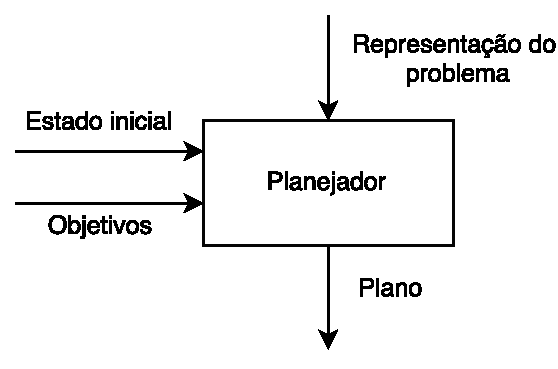
\includegraphics[width=0.4\textwidth]{fig/modelo.pdf}
	\caption{Modelo de estado e transição}
	\label{fig:planmodelo}
\end{figure} 

Um plano é gerado, quando dado um estado inicial e um objetivo, um conjunto de ações é gerado e quando executadas levam ao objetivo. O processo usado para conseguir isso é chamado de planejamento, onde é necessário ter uma descrição do sistema($\sum$) onde os estados e as ações são definidos.\\ 
Os estados são representados por um conjunto de átomos sem função \cite{intelligence2003modern}, que são usados para representar alguma situação, por exemplo uma pessoa estar em um lugar pode ser representado por \textit{at(Matheus, PUCRS)}, assim todos os estados devem seguir o padrão, podendo ter mais de uma situação, como por exemplo, representar que alguém está em um lugar e feliz ao mesmo tempo, \textit{at(Matheus,PUCRS) $\wedge$ happy(Matheus)}. \\
As ações são descritas por um conjunto esquema de ações \cite{intelligence2003modern}. Para toda ação é necessário uma pré condição aplicada ao estado atual, que se for satisfeita, garante o efeito ou pós condição, levando o sistema para o estado resultante. Por exemplo, caminhar de um lugar a outro: \\
\textit{Action(walk(from, to)): \\
Precond: at(from)  $\wedge$ path(from,to) \\
Effect: $\neg$ at(from)  $\wedge$ at(to)}

\subsection{HTN} 
Dentro do planejamento existe um tipo especifico chamado \textit{Hierarchical Task Network Planning} (HTN). Os métodos de HTN são utilzados pelo fato do problemas serem descrito como receitas, seguindo uma ordem de execução das tarefas, que pode corresponder como pessoas pensam em resolver problemas de planejamento \cite{ghallab2004automated}.  \\
A grande diferença de planejamento HTN dos demais tipos de planejamento é o fato de que as ações são tratadas em mais alto nível \cite{intelligence2003modern}. As ações vão sendo decompostas até serem diretamente executadas, um bom exemplo é viajar de avião, a tarefa principal é viajar de um lugar para o outro, mas antes disso deve-se comprar a passagem e ir até o aeroporto de táxi para então conseguir realizar a viagem. 

Em HTN as ações são chamadas de tarefas e a finalidade não é alcançar o objetivo, e sim realizar um conjunto de tarefas que resolvam um determinado problema. Como entrada para o sistema é necessário um conjunto de operadores e um conjunto de métodos. Em HTN as ações são chamadas de tarefas, e podem ser dividas em dois tipos: Primitivas e não primitivas. As tarefas primitivas são executadas diretamente através do conjunto de métodos, já as tarefas não primitivas são decompostas recursivamente em sub tarefas e assim se transformando em tarefas menores até se tornarem em tarefas primitivas, e assim podem ser executadas. A figura \ref{fig:travelmethods} mostra um exemplo de descrição dos métodos para uma viagem de avião.

\begin{figure}[ht]
	\centering
	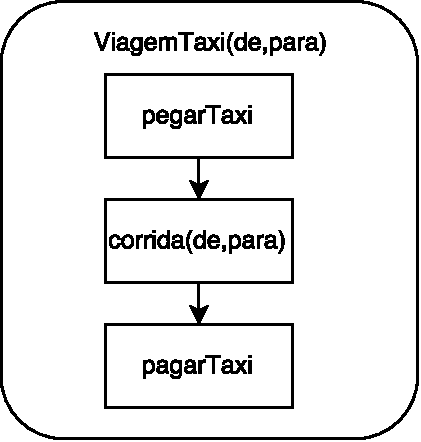
\includegraphics[width=0.8\textwidth]{fig/travelmethod.pdf}
	\caption{Exemplo de problema de HTN}
	\label{fig:travelmethods}
\end{figure}  

O planejamento HTN executa todas as possibilidades de resolução do problema, sempre respeitando a ordem dos métodos que conseguem ser realizados, quando um caminho de resolução leva a um fim de linha é realizado um retrocesso(\textit{backtracking}) até um caminho que tenha uma possibilidade de caminho diferente do que foi tomado anteriormente.

\subsection{AHTN} 

%AHTN é HTN + game tree search \cite{adversal}
\textit{Adversarial hierarchical-task network} (AHTN) é um algoritmo proposto para tentar solucionar o problema do grande fator de ramificação dos jogos em tempo real \cite{ontanon2015adversarial}. O algoritmo combina técnicas de planejamento HTN e o algoritmo \textit{minimax game tree search}. \\
%explicar Game search tree(minimax)
%explicar técnica de HTN utilizada
%explicar diferença do minimax puro

\subsection{Motivação e aplicação}
A motivação para o estudo de planejamento automatizado vem do fato que, como planejamento é um componente vital do comportamento racional, e a IA busca alcançar aspectos de inteligencia a nível computacional, então planejamento é um elemento chave para isso\cite{ghallab2004automated}.
%algumas aplicações de planejamento e exemplos

\section{Aprendizado} 
%-overview de aprendizado
%**O que é em geral \\
Para os humanos o aprendizado ocorre durante toda a vida. O aprendizado é o ato de adquirir novos conhecimentos, ou modificar conhecimentos já existentes ou ainda adquirir uma experiencia por repetição do ato de forma incorreta. Aprendizado pode variar de adquirir conhecimento de tarefas simples, como decorando um numero de telefone, até tarefas mais complicadas, como a formulação de novas teorias \cite{intelligence2003modern}. \\
Na computação o aprendizado depende de alguns fatores \cite{intelligence2003modern}:
\begin{itemize}
	\item Qual o conhecimento que será melhorado ou descoberto.
	\item Qual o conhecimento que o sistema já possui.
	\item Qual é a representação usada por esse conhecimento.
	\item Qual é o aprendizado disponível de fato.
\end{itemize}


\subsection{Aprendizado de Máquina} 

% o que é aprendizado de maquina
% Definição de ML: aprende atráves de um experiencia E em uma tarefa T com uma performace P  
% reinforcement o que é - aprendizado atráves de um conjunto de simulações
% explicar Q LEARNING

\subsection{Motivação e aplicação}
%motivação
%aplicação no mundo real com exemplos


%\section{Jogos Real-time Strategy(RTS)} 

%Jogos eletrônicos são muito populares, não só entre os jovens, principalmente pela grande quantidade de gêneros, existem jogos de ação, aventura, esportes, estrategia, entre outros. \\
%Dentro dos jogos de estratégia há uma subseção que se chama jogos de estratégia em tempo real, neles os jogadores estão se enfrentando no mesmo momento, como o nome já diz. Em alguns desses jogos há BOTs(jogadores que simulam um jogador real) e é preciso alguma inteligencia para esses BOTs conseguirem levar graça ao jogador real, para isso é utilizado algoritmos de IA. Esse tipo de jogo, devido a sua grande quantidade de ações, possui um fator de ramificação muito grande, e cresce exponencialmente, com isso aplicar os algoritmos se torna uma tarefa não trivial.  \\
%!TEX root = volumeFinal.tex 
\chapter{\label{chap:agentes}Agentes} 

\frm[inline]{De repente reestruturar um pouco esta seção para falar de agentes e jogos e começar com uma motivação mais complexa ao invés de só dropar a frase dos agentes nos jogos...}

\frm[inline]{Vi que tu utiliza bastante referências ao livro do Norvig~\cite{intelligence2003modern}, isto não é ideal para tudo, mas é aceitável em alguns lugares. \textbf{Só que}, quando referenciar um livro \textbf{sempre} usar o parâmetro opcional do \texttt{{\textbackslash}cite[opcional]\{key\}} para indicar o \textbf{capítulo} que tu te refere, senão a referência não ajuda o leitor em nada.}

Os agentes são utilizados em jogos como uma abstração que represente os jogadores. Os agentes conseguem absorver informações providas do jogo e assim decidir qual o próximo passo a ser tomado \cite{millington2009artificial}. 

Formalmente, agentes são entidades que agem de forma continua e autônoma em um ambiente \cite{agent1993oriented}. 
Os agentes são capazes de receber estímulos do ambiente através de sensores, e assim responder aos estímulos por intermédio de atuadores. 
Para os agentes os estímulos do ambiente são recebidos como percepções. 
Os atuadores por sua vez, geram, uma ação considerando as percepções~\cite{intelligence2003modern}. 
A interação de um agente com o ambiente pode ser ilustrado pela Figura~\ref{fig:agente}.

\begin{figure}[ht]
	\centering
	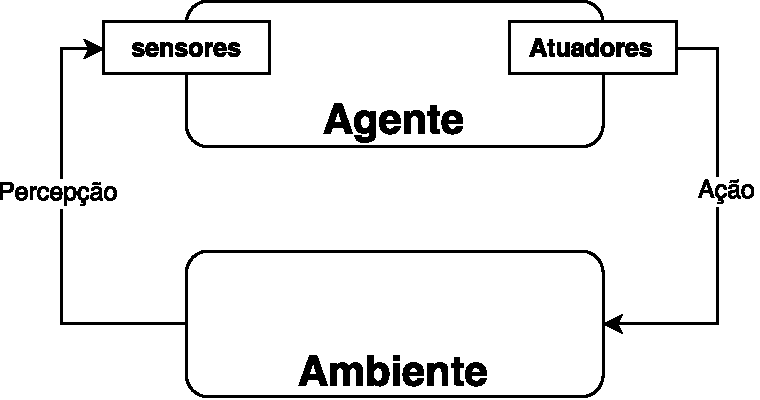
\includegraphics[width=0.5\textwidth]{fig/agente.pdf}
	\caption{Representação de um agente}
	\label{fig:agente}
\end{figure} 

O agente deve agir de forma autônoma, para isso ele deve ser capaz de aprender a lidar com situações proporcionadas pelo ambiente, com o intuito de realizar ações em busca do seu objetivo. O agente precisa de três características para conseguir ser autônomo \cite{agent1999}. São elas:
 
\begin{itemize}
	\item reatividade, para que os agentes sejam capazes de perceber o ambiente e suas mudanças a fim de levar o ambiente em consideração para a tomada de decisão das ações;
	\item pró-atividade, para que os agentes consigam ter a iniciativa em tomar as suas ações; e
	\item habilidade social, para que os agentes sejam capazes de interagir com outros agentes(humanos ou não).
\end{itemize}

As duas primeiras características são necessárias para que o agente consiga interagir com o ambiente. Um agente sendo reativo, ele consegue, a partir de uma mudança do ambiente, saber como ele deve se comportar. Sendo proativo, o agente pode antecipar suas ações em busca do seu objetivo.
Nem sempre um agente vai estar sozinho no ambiente, por esse motivo, a terceira característica é necessária para que o agente consiga interagir com outros agentes. Sistemas onde existem mais de um agente são chamados de sistema multi agentes. Nesses sistemas, os agentes interagem entre si, podendo ter objetivos em comum ou não. Sendo assim eles terão que cooperar ou negociar entre si \cite{intelligence2003modern}.

\section{Ambientes}

O agente deve se comunicar com um ambiente para conseguir alcançar seus objetivos. Mas um ambiente é composto por diversas propriedades que podem influenciar como o agente vai agir para chegar ao seu objetivo \cite{intelligence2003modern}. 

Nem sempre todas as informações do ambiente estarão disponíveis, por esse motivo o ambiente pode ser dito como completamente observável, parcialmente observável ou não observável, dependendo da informação disponibilizada. Um ambiente é dito completamente observável se, em qualquer instante de tempo, todas as informações relevantes do ambiente estão disponíveis para os sensores do agente. Caso haja alguma informação que não possa ser acessada, em algum instante de tempo, seja por causa da incapacidade do sensor do agente de captar essas informações ou pelo fato da informação simplesmente não ser disponibilizada, o ambiente é dito parcialmente observável. Agora, se o ambiente não disponibiliza nenhuma informação, o ambiente é tido como não observável \cite{ intelligence2003modern, agent1999}.   

O ambiente pode sofrer modificações, as modificações podem ser provenientes de ações realizadas pelos agentes, ou ainda por mudanças ocasionadas pelo próprio ambiente. O ambiente é determinístico se o estado gerado após a execução de uma ação, em todas as vezes que for executada, levar para o mesmo estado resultante, ou seja, o estado resultante é determinado pelo estado atual e a ação executada pelo agente. Se não há a certeza do estado resultante, o ambiente é estocástico. Quando o ambiente é não determinístico existem chances das ações dos agentes nem lembre levarem para os estados conhecidos \cite{intelligence2003modern}. 

Os estados do ambiente irão mudar ao longo do tempo, seja por uma ação feita por algum agente, ou por alguma mudança que possa ocorrer em razão de outro processo do ambiente. Se o ambiente sofre alguma alteração apenas quando o agente executa alguma ação, o ambiente é estático. Se o ambiente tem a capacidade de mudar independente de uma ação de um agente, o ambiente é dinâmico \cite{agent1999}.

Em sistemas multi agentes os agentes podem estar competindo ou cooperando entre si. O ambiente é competitivo quando os agentes estão competindo, como em um jogo de xadrez, por exemplo, ou o ambiente é cooperativo quando os agentes estão cooperando \cite{intelligence2003modern}.

\section{Arquiteturas de Agentes}


O tipo mais simples de agente é aquele que apenas reage a uma percepção vinda do ambiente. O agente escolhe suas ações baseado no que percebe no momento da decisão, sem levar em consideração ações já tomadas ou percepções anteriores. O agente apenas responde a uma percepção com uma ação, como se houvesse um clausula condicional que determinasse qual a ação a ser tomada se acontecer alguma coisa, como por exemplo, se estiver chovendo eu irei levar um guarda-chuva. A Figura~\ref{fig:agenteSimple} ilustra essa arquitetura. 

\begin{figure}[ht]
	\centering
	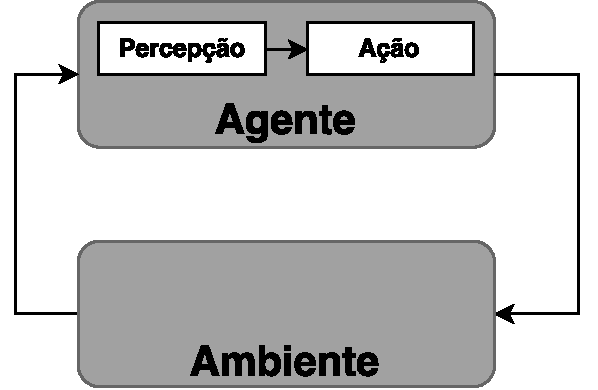
\includegraphics[width=0.4\textwidth]{fig/agentSimple.pdf}
	\caption{Arquitetura simples de um agente.}
	\label{fig:agenteSimple}
\end{figure} 


Este tipo de agente consegue ser simples, no entendimento e na sua utilização, mas a sua inteligência é limitada. Essa arquitetura é eficaz em ambientes completamente observáveis, pelo fato de que o agente precisa da percepção para realizar a sua ação \cite{intelligence2003modern}. A arquitetura pode ser usada, por exemplo, quando for preciso conhecer um conjunto de cidades, o agente após chegar a uma cidade, vai para a próxima cidade ao norte da cidade atual, quando não há norte ele vai para oeste. 

Na tentativa de aprimorar as decisões tomadas pelo agente, pode-se usar um estado interno para marcar qual a situação do ambiente. A informação representada no estado pode ser alguma informação que não consiga ser obtida por alguma percepção do ambiente ou de estados que já foram visitados pelo agente, por exemplo \cite{intelligence2003modern}. A Figura~\ref{fig:agenteModelbased} ilustra esta arquitetura. 

\begin{figure}[ht]
	\centering
	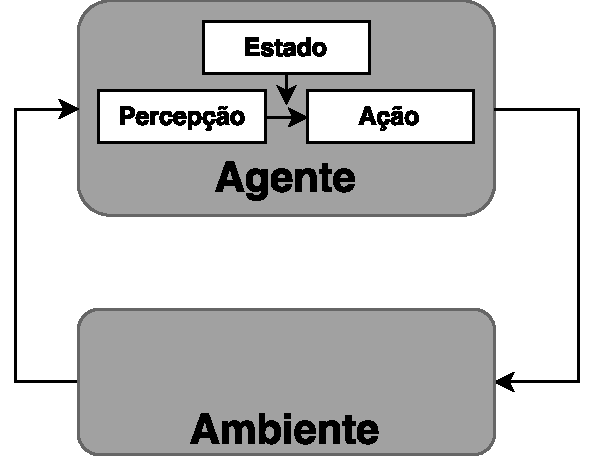
\includegraphics[width=0.4\textwidth]{fig/agentModel.pdf}
	\caption{Arquitetura de agentes com estados.}
	\label{fig:agenteModelbased}
\end{figure} 

Este tipo de arquitetura é eficaz para ambientes parcialmente observáveis, pelo fato de que o estado pode guardar informações relevantes para o agente \cite{intelligence2003modern}. No exemplo de conhecer as cidades, se guardar as visitas antigas, pode ajudar a não visitar novamente cidades que já tiverem sido visitadas. 

Dependendo do intuito do agente, conhecer o estado atual do ambiente não é suficiente. Além de estado, o agente pode precisar de uma informação para saber onde ele quer chegar, ou seja, um objetivo. Um objetivo é usado para descrever o que o agente está almejando alcançar. Para o agente conseguir alcançar o objetivo com uma melhor performance pode ser utilizado uma função de utilidade, nesta função é medido o "desejo" do agente em tomar determinada ação. Cada ação exercida pelo agente terá influência no valor de utilidade obtido \cite{intelligence2003modern}. Seguindo no exemplo, o objetivo pode ser visitar todas as cidades e a função de utilidade pode medir a distância entre as cidades, e assim podendo alcançar o objetivo com a menor distância percorrida. 



%!TEX root = volumeFinal.tex 
\chapter{\label{chap:busca}Busca}

Com o intuito de encontrar uma sequência de ações que um agente consiga alcançar o seu objetivo, é possível utilizar técnicas de busca.
O princípio da busca é encontrar uma solução de um problema através de um conjunto de ações que alcancem o objetivo desejado. 
Para utilizar as técnicas de busca é preciso formalizar o problema a ser resolvido e o objetivo a ser alcançado. Para utilizar as técnicas de busca, como entrada é recebido um problema e como resolução é retornado um conjunto de ações. 
Um problema pode ser definido por cinco componentes \cite{intelligence2003modern}: 

\begin{itemize}
	\item $s_{0}$, o estado inicial, onde o agente inicia no ambiente;
	\item ações, conjunto das possíveis ações disponíveis no agente;
	\item $resultado(s, a)$, um modelo de transição, que define o estado resultante após a execução da ação a no estado s;
	\item $objetivo(s)$, verifica se o estado é o objetivo do agente; e
	\item custo do caminho, uma função que define um valor numérico para cada ação realizada em um estado. Essa função pode ser denotada por $c(s, a, s')$, onde s é o estado atual do agente, a é a ação que será aplicada ao estado s e $s'$ é o estado resultante aplicando o modelo de transição resultado(s, a). 
\end{itemize}   


Esses elementos são necessários como entrada para que as técnicas de busca consigam ser utilizadas. As técnicas de busca visam encontrar a solução para esse problema, ou seja, a sequência de ações que leve ao objetivo. 
A solução é obtida quando o agente iniciando no estado inicial do ambiente $s_{0}$, utiliza o modelo de transição $resultado(s, a)$, através das ações aplicadas nos estados, para chegar a um estado onde satisfaça o objetivo do agente $objetivo(s)$.
Existem diferentes técnicas para encontrar uma solução. As diferentes técnicas podem encontrar caminhos diferentes para o mesmo problema, isso vem do fato de que o custo do caminho, quando levado em consideração, pode encontrar uma solução ótima, o que significa que a sequência de ações encontrada é a que tem o menor custo de caminho entre todas as soluções \cite{intelligence2003modern}.

Com a finalidade de exemplificar um problema de busca, considere o mapa apresentado na figura \ref{fig:mapabusca}. Cada círculo representa uma cidade, e as linhas entre as cidades são estradas que ligam as cidades uma a outra. A única ação possível é a de se locomover entre as cidades que tenham ligação. O estado inicial é a cidade de São Jerônimo. O resultado do modelo de transição, é a cidade resultante após se locomover. O objetivo do agente é chegar na cidade de Porto Alegre e o custo de cada ação é o valor definido em cima de cada transição. 

\begin{figure}[ht]
	\centering
	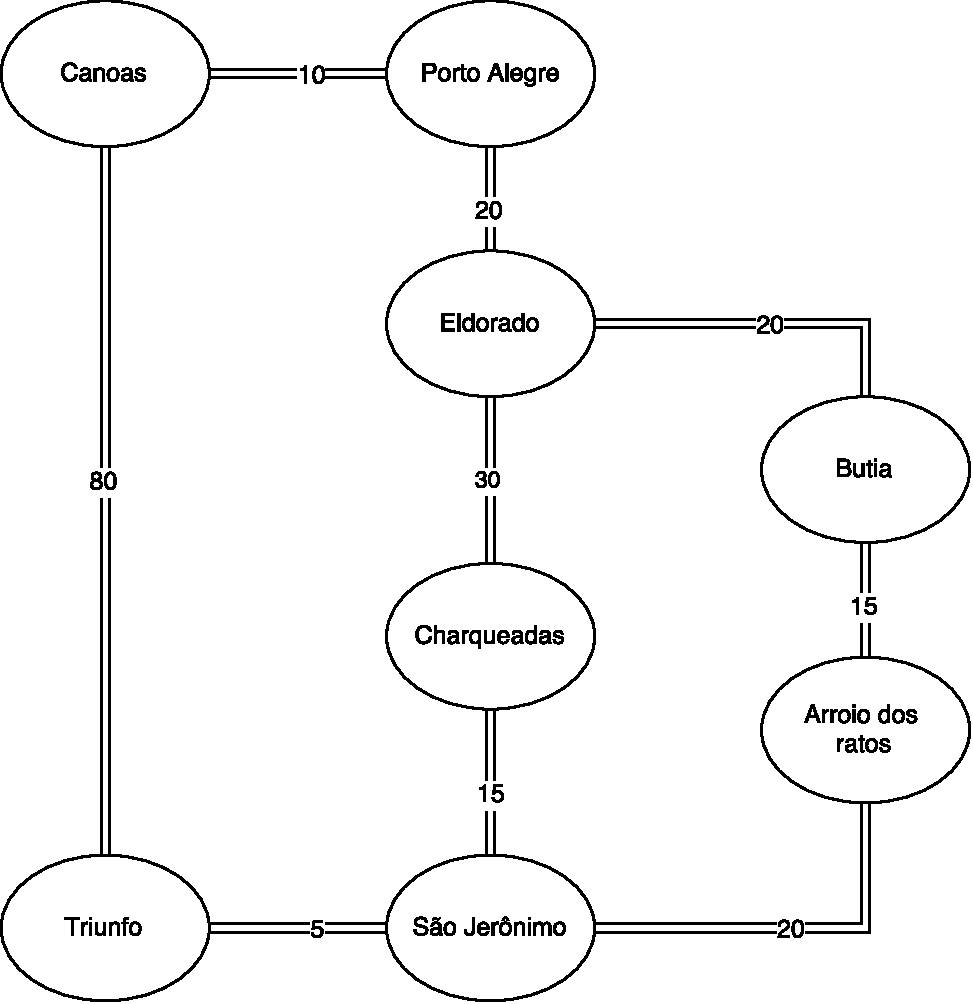
\includegraphics[width=0.6\textwidth]{fig/mapabusca.pdf}
	\caption{Mapa para o exemplo de problema de busca}
	\label{fig:mapabusca}
\end{figure} 

Para atingir o objetivo é preciso tentar os possíveis caminhos até o objetivo. Digamos que o agente comece sua viagem indo para a cidade de Triunfo, para nós(humanos) é intuitivo que a escolha não foi a melhor escolha para iniciar, mas a técnica só terá como saber após realizar todas as possíveis opções de caminhos, ou se utilizar uma técnica que utilize uma função de heurística, levando em consideração os custos dos caminhos, que acrescentam um conhecimento extra para a resolução do problema \cite{intelligence2003modern}.

\section{Busca adversaria}

Jogos são difíceis de resolver com técnicas de IA, pois eles requerem a habilidade de tomar algum tipo de decisão, e as técnicas comuns as vezes não são satisfatórias, seja pelo fato do conjunto de estados possíveis de se atingir ser muito grande, ou pelo curto espaço de tempo para tomar essa decisão.
A busca adversaria é utilizada nos jogos que estão situados em ambientes competitivos e de multi agentes. Em um jogo o jogador, preferencialmente, não informa suas jogadas previamente, assim tornando o ambiente imprevisível. Os objetivos dos jogadores entram em conflito, pois ambos estão em busca da vitória. 
Com o intuito de resolver esse problema é possível gerar uma solução de contingência para tentar antecipar as jogadas do adversário \cite{intelligence2003modern}. 

As técnicas de busca adversária utilizam uma variação da definição de um problema de busca comum. Os componentes devem se adequar ao ambiente competitivo. Por esse motivo os componentes são redefinidos como:

\begin{itemize}
	\item $s_{0}$, sendo o estado inicial, que especifica como o jogo se configura no início;
	\item $players(s)$, define qual jogador tem o movimento no estado $s$;
	\item $actions(s)$, conjunto das ações possíveis em um estado $s$;
	\item $result(s, a)$, um modelo de transição, que define o resultado da ação $a$ a aplicada ao estado $s$;
	\item $terminal(s)$, verifica se o estado $s$ é um estado onde o jogo termina; e
	\item $utility(s,p)$, define um valor numérico, representando o lucro do jogador $p$ ao atingir o estado terminal $s$.
\end{itemize}

Com esses componentes descritos é possível formalizar o que é uma árvore de jogadas. A árvore de jogados ou \textit{game tree} contém os estados do jogo e os movimentos possíveis em cada estado. A \textit{game tree} é composta pelo estado inicial $s_{0}$, as ações $action(s)$ e o modelo de transição $result(s, a)$, e possui uma profundidade $d$, que indica o nível máximo da árvore. 
A árvore representa em cada nodo um estado do jogo e em cada ligação os estados resultantes após a execução de cada ação possível para o estado. Considerando o jogo de jogo da velha, onde cada jogador realiza uma jogada de cada vez, uma \textit{game tree} que mostra parte das jogadas do jogo da velha é ilustrada na Figura~\ref{fig:jogodavelha}. O estado inicial do jogo é o campo vazio, a cada nível da árvore todas as possibilidades de jogadas são testadas, a profundidade $d$ dessa árvore chega a 9 quando ela estiver completa, pois a cada nível da árvore uma jogada é marcada no campo. 

\begin{figure}[ht]
	\centering
	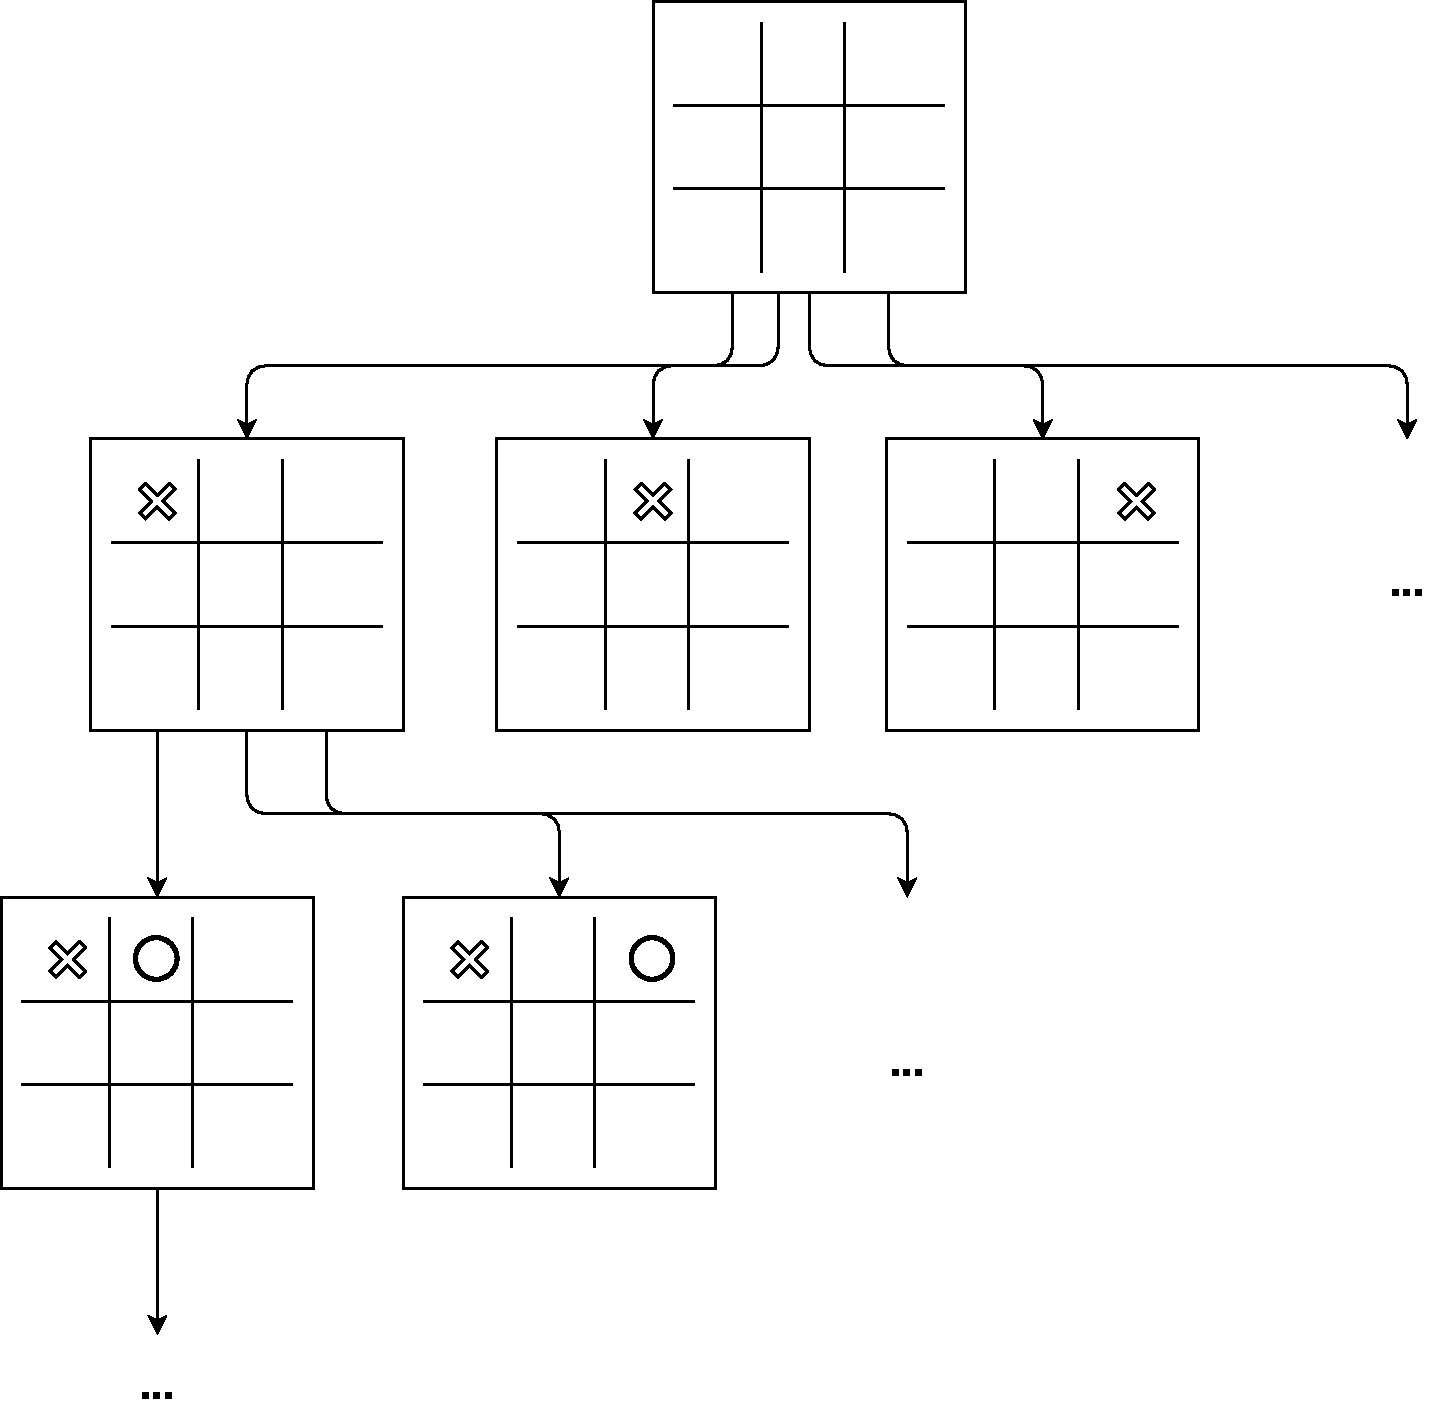
\includegraphics[width=0.5\textwidth]{fig/jogodavelha.pdf}
	\caption{Exemplo de um pedaço de uma \textit{game tree} sobre o jogo da velha}
	\label{fig:jogodavelha}
\end{figure} 

\section{Minimax search}

O algoritmo de \textit{minimax search} é utilizado como uma técnica de busca adversária. O objetivo do algoritmo é retornar a melhor jogada para o estado atual. Esse método considera dois agentes, chamados de \textsc{Max} e \textsc{Min}, onde o jogador \textsc{Max} representa a perspectiva do agente que está tentando maximalizar suas ações em relação ao agente \textsc{Min}, que representa o agente adversário do jogador \textsc{Max}. O algoritmo alterna entre jogadas de \textsc{Max} e \textsc{Min} \cite{intelligence2003modern}. 

O algoritmo utiliza a \textit{game tree} para analisar todos os estados possíveis do jogo, e assim decidir qual a ação que quando aplicada ao seu estado atual, trará um melhor benefício no futuro, se caracterizando a melhor jogada. Os nodos folhas da árvore, que representam o final do jogo, contém um valor de utilidade. Os valores mais altos são as melhores jogadas para \textsc{Max}, e consequentemente, os valores menores são melhores para \textsc{Min}. Ao chegar no final da árvore o algoritmo consegue o valor de utilidade para aquele cenário do jogo, quando isso acontece, o algoritmo faz o caminho inverso na árvore analisando os outros possíveis cenários \cite{intelligence2003modern}. A Figura~\ref{fig:gametree} ilustra esse processo.

\begin{figure}[ht]
	\centering
	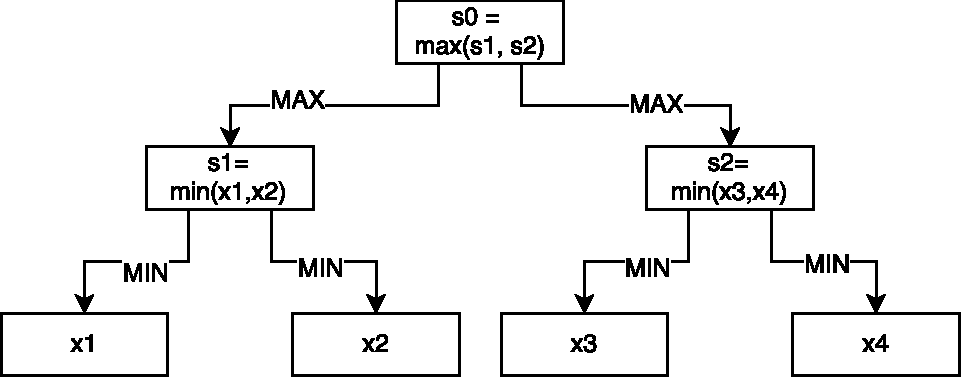
\includegraphics[width=0.6\textwidth]{fig/gametree.pdf}
	\caption{Exemplo de game tree utilizando \textit{minimax search}}
	\label{fig:gametree}
\end{figure} 

O método de \textit{minimax search} assume que os todos os jogadores como sendo racionais, com isso o algoritmo considera que as ações tomadas pelos agentes sempre realizarão uma jogada para tentar ganhar o jogo. O algoritmo de \textit{minimax search} é ilustrado no Algoritmo~\ref{alg:minimax}. O algoritmo tem como retorno a melhor ação a ser realizada no estado atual. As funções presentes nas linhas~\ref{alg:minimax:max} e ~\ref{alg:minimax:min} são utilizadas para calcular a jogada na visão de \textsc{Max} e \textsc{Min} respectivamente.
A função presente na linha~\ref{alg:minimax:minimax} é utilizada para iniciar a recursão e ao final retornar o melhor valor de utilidade para o jogador \textsc{Max}.

\begin{algorithm}
	\caption{Minimax Search}
	\label{alg:minimax}
	\begin{algorithmic}[1]	
		\Function{Minimax}{$state$} \label{alg:minimax:minimax}
		\State \Return $arg max_{action~ \in~ actions(s)}~ min\_value(result(state,  action)) $
		\EndFunction \\
		\Function {Max\_Value}{$state$}\label{alg:minimax:max}
		\If {$terminal(state)$}
		\State	\Return $utility(state)$
		\EndIf
		\State $v = -\infty$
		\ForAll{$action \in actions(state)$}
		\State $v = max(v, min\_value(result(state,action)))$
		\EndFor	
		\EndFunction \\
		\Function {Min\_Value}{$state$}\label{alg:minimax:min}
		\If {$terminal(state)$}
		\State	\Return $utility(state)$
		\EndIf
		\State $v = \infty$
		\ForAll{$action \in actions(state)$}
		\State $v = min(v, max\_value(result(state,action)))$
		\EndFor	
		\EndFunction
	\end{algorithmic}
\end{algorithm}


O algoritmo de \textit{minimax} deve explorar todo o espaço de estados para conseguir encontrar a ação que deve ser executada. A quantidade de estados possíveis, dependendo da situação, pode ser muito alta, no xadrez esse número chega a $10^{50}$, em um jogo de \textit{poker} no estilo \textit{texas holdem} esse número pode chegar a $10^{80}$. Geralmente, as ações devem ser tomadas em uma quantidade de tempo muito pequena. Por esse motivo, utilizar técnicas de busca para jogos pode ser um problema. Existem algumas abordagens que utilizam busca adversaria com um nível de abstração mais alto para tentar minimax esse problema \cite{ontanon2013survey}. 
%!TEX root = volumeFinal.tex 
\chapter{Planejamento}
\label{chap:planejamento}

A atividade de planejar alguma coisa é feita muitas vezes por dia. Algumas vezes esse planejamento é muito simples, como organizar as tarefas que serão feitas no próximo dia, outras vezes pode ser mais complexa como organizar uma viagem de final de ano. Planejar implica em elaborar uma sequência de ações com o intuito de alcançar um objetivo, ou seja, o processo de planejar consiste em organizar as ações, antecipando os resultados esperados de cada ação, com o intuito de conquistar um objetivo. 

O planejamento, na área da IA, é uma sub área de estudo, onde ele é usado para encontrar um plano que resolva um problema especifico. Como os ambientes nem sempre possuem as mesmas características, existem diferentes técnicas que são usadas para construir um plano.

\section{Planejamento automatizado}
\label{sec:classicalPlanning}

Planejamento automatizado estuda o processo de geração de planos computacionalmente. O objetivo do planejamento é encontrar uma sequência de ações que solucione um problema, a sequência de ações encontrada é chamada de plano. Para construir um plano é utilizado um planejador. O planejador recebe uma descrição formal de um problema de planejamento, e tenta solucionar esse problema, para isso pode ser utilizado algoritmos de buscas e heurísticas~\cite{ghallab2004automated}\cite[Capítulo 10]{intelligence2003modern}.

\subsection{Representação de um problema de planejamento}
\label{subsec:classicalPlanningRep}

Uma das maneiras de representar um problema de planejamento é utilizando lógica proposicional.
A lógica proposicional é expressada através de sentenças atômicas, que são compostas de proposições. 
Cada proposição pode assumir um valor de verdadeiro ou falso. 
Por exemplo, queremos representar que a lâmpada está apagada, para isso pode ser utilizado a proposição $apagada$, se a lâmpada estiver apagada, a proposição assume o valor de verdadeiro. Junto com as proposições podem ser usados conectivos lógicos, como negação (\textit{not}) $\neg$, conjunção (\textit{and}) $\wedge$ e disjunção (\textit{or}) $\vee$. 
No exemplo da luz, se queremos saber se a luz está apagada e a TV está ligada, podemos representar por $apagada~ \wedge~ ligada$. 
A lógica proposicional pode ser considerada simples, mas ela serve de base para as lógicas mais expressivas~\cite[Capítulo 10]{intelligence2003modern}. 

Como a lógica proposicional tem expressividade limitada, é preciso utilizar uma lógica que consiga expressar mais sobre os estados do ambiente que desejamos representar. 
A lógica de primeira ordem (LPO) estende a lógica proposicional, e diferente da lógica proposicional a LPO consegue representar relação entre preposições, ou seja, as preposições podem ter aridade mais que um, um exemplo pode ser um objeto estar sobre o outro ($sobre(A,B)$). Uma outra diferenças da LPO é a possibilidade de utilizar quantificadores para demonstrar fatos comuns sobre as preposições, como objetos que tenham a mesma cor ($\forall x~ azul(x)$).

A descrição formal de sentenças em LPO é composta por um predicado seguido de uma lista de termos, denotada por $p(t_{0}, t_{1}, ..., t_{n})$. 
Um predicado se refere a uma relação existente entre os termos. 
Os termos são objetos que se referem a objetos definidos, indefinidos ou a funções \cite[Capítulo 10]{intelligence2003modern}. 
No exemplo da lâmpada, podemos dizer que a lâmpada da cozinha está apagada, representado por $apagada(cozinha)$. 
Ou ainda podemos dizer que a lâmpada do quarto está apagada e a TV da sala está ligada, $apagada(quarto)~ \wedge~ ligada(sala)$.  

\subsection{Formalização de um problema de planejamento}
\label{subsec:classicalPlanningForm}

Alguns conceitos são importantes para entender a formalização de um problema de planejamento. 
Os estados são um conjunto de átomos que não podem ser divididos em sub-fórmulas, esses átomos assumem valores de verdadeiro ou falso, dependendo da interpretação do ambiente.
As ações alteram o estado do ambiente. Para que elas sejam aplicadas é preciso que um conjunto de precondições seja satisfeito, se for é aplicado um conjunto de efeitos sobre o ambiente~\cite[Capítulo 10]{intelligence2003modern}.
Um exemplo é mover um objeto de um lugar para o outro, precisamos de um predicado que defina que um objeto está em determinado lugar. Esse exemplo é representado abaixo:

\begin{itemize}
	\item Ação: $move(from, to)$
	\item Precondição: $at(from)$
	\item Efeito: $\neg at(from) \wedge at(to)$
\end{itemize}

Uma ação $a$ é aplicável em um estado $s$, se todas as precondições forem satisfeitas no estado $s$. 
O resultado gerado pela execução de $a$ no estado $s$ é um novo estado $s'$, nesse estado é aplicado todos os efeitos, removendo os predicados negativos e adicionando os positivos~\cite{meneguzzi2015planning}.

Os operadores são definido como $op = (nome(t), precondições(p), efeitos(p)$. 
O $nome(t)$ é o nome do operador e $t$ é o conjunto de termos que compõem as precondições e os efeitos. $precondições(p)$ é o conjunto de predicados que representam as precondições do operador. $efeitos(p)$ é o conjunto de predicados que serão o resultado após a execução do operador;
Todas os operadores disponíveis para a resolução do problema formam a descrição das ações~\cite{ghallab2004automated}.
 
Como nas técnicas de busca, em planejamento também é necessário ter uma descrição do problema.
Formalmente, um problema de planejamento pode ser descrito como $P = (\Sigma, s_{0}, g)$, onde $\Sigma$ é a descrição do problema com as ações disponíveis, $s_{0}$ é o estado inicial onde o problema começa e $g$ é o objetivo~\cite{ghallab2004automated}. 
Voltando ao exemplo do Capítulo~\ref{chap:busca}, onde um agente tenta chegar a cidade de Porto Alegre partindo da cidade de São Jerônimo, podemos formalizá-lo como:

\begin{itemize}
	\item \textbf{estado inicial} ($s_{0}$) = $At(S$\~a$o~Jer$\^o$nimo)$;
	\item \textbf{objetivo} ($g$) = $At(Porto~Alegre)$; e
	\item \textbf{domínio} ($\Sigma$) = 
	\begin{itemize}
		\item nome: $move(cityA, cityB)$
		\item precondições: $at(cityA) \wedge link(cityA, cityB)$
		\item efeitos: $\neg at(cityA)~ \wedge at(cityB)$.
	\end{itemize}
\end{itemize}


O processo de geração do plano é feito pelo planejador. 
Um plano é uma sequência de operadores gerada a partir de um problema que, quando executada partindo do estado inicial, modifica o estado de forma que o objetivo seja válido no estado resultante. 
A Figura~\ref{fig:planmodelo} ilustra o comportamento do planejador.
Para realizar a formalização de um problema de planejamento é preciso definir alguns conceitos.

\begin{figure}[ht]
	\centering
	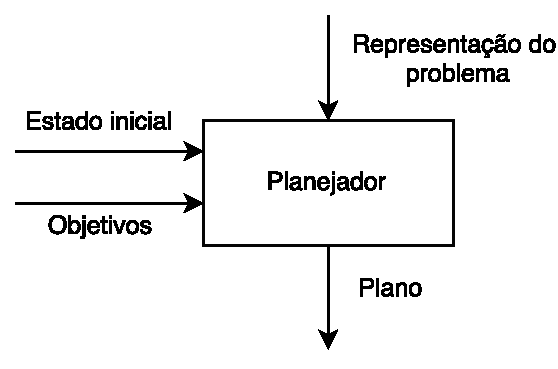
\includegraphics[width=0.4\textwidth]{fig/modelo.pdf}
	\caption{Problema de planejamento clássico.}
	\label{fig:planmodelo}
\end{figure} 

Um plano é considerado ótimo quando não há nenhum outro plano que atinga o objetivo utilizando um número menor de ações.
Uma forma de gerar planos ótimos é utilizando técnicas de busca combinado com alguma heurística que seja independente de domínio.
Uma heurística deve ser computacionalmente eficiente e ter precisão para que a geração do plano seja eficiente~\cite{helmert2007flexible}.

\section{Planejamento hierárquico} 
\label{sec:htnPlanning}

O planejamento clássico consegue gerar planos ótimos.
Mas o tratamento de problemas de grande complexidade ou com o espaço de estados grande pode se tornar intratável.
Isso acontece por conta do poder computacional necessário para que o plano consiga ser gerado.
O planejamento clássico possui uma expressividade limitada, pois não é possível representar quando uma ação irá ocorrer, por exemplo~\cite[Capítulo 11]{intelligence2003modern}.
Como alternativa para esses problemas foi proposto o planejamento hierárquico, chamado de \textit{Hierarchical Task Network} (HTN). 
O planejamento HTN se diferencia do planejamento clássico na forma como os planos são gerados~\cite{ghallab2004automated}. 
Enquanto no planejamento clássico é necessário ter heurísticas para a geração de planos, em planejamento HTN é possível expressar conhecimento de domínio junto com os operadores, isso faz com que as ações sejam tratadas em mais alto nível.  
O conhecimento de domínio contém informações que determinam o espaço de estados possível para determinado ambiente. O planejador utiliza o conhecimento de domínio para percorrer entre os estados e encontrar os planos possíveis. Para isso o conhecimento de domínio deve conter informações relativas as ações, disponíveis no ambiente, e as possíveis transições de estados~\cite[Capítulo 11]{intelligence2003modern}.

O objetivo do planejamento HTN é produzir uma sequência de ações que executam determinada tarefa $t$. 
As tarefas são completadas decompondo tarefas não primitivas em tarefas menores até só restarem tarefas primitivas.  
As tarefas primitivas são análogas as ações executáveis em planejamento clássico, e expressam uma atividade que o agente possa executar diretamente no ambiente~\cite[Capítulo 11]{intelligence2003modern}. 
Já as tarefa não primitiva representam objetivos que o agente deve alcançar com o intuito de decompor as tarefas não primitivas em primitivas. 
O exemplo da seção anterior de mover um objeto de lugar é um exemplo de tarefa primitiva, pois altera o estado do ambiente, podendo ser representado em HTN como: \texttt{(move~ ?from~ ?to)}. 
Um exemplo de tarefa não primitiva é realizar uma viagem de carro, para conseguir completar essa tarefa é necessário fazer a revisão do carro, arrumar as malas e colocar tudo dentro do carro, que pode ser representado por \texttt{(travelByCar ~?car~ ?stuffs)}. 

Para iniciar a geração de um plano HTN, deve ser usado como início uma tarefa de ligação. 
Uma tarefa de ligação HTN é definida como $w = (T, C)$, onde $T$ é um conjunto de tarefas a ser completadas e $C$ é um conjunto ordenado de restrições sobre as tarefas $T$. 
As restrições estabelecem a ordem com que as tarefas $T$ devem ser executadas. 

Um domínio de planejamento HTN é um par $D = (A, M)$, onde $A$ é um conjunto de predicados, que representam estados no ambiente, e $M$ um conjunto finto de métodos \cite{meneguzzi2015planning}. 
Um método é utilizado para decompor tarefas não-primitivas em primitivas. 
Um método é representado por $m = (p, t, w)$, onde $p$ é uma precondição que estabelece o que deve estar presente no estado atual para que a tarefa $t$ consiga ser decomposta por uma tarefa de ligação $w$ \cite{ghallab2004automated}. 
Considerando o exemplo anterior de viajar de carro, a Figura~\ref{fig:htnmethod} ilustra esse método, sendo a tarefa em cinza uma tarefa não primitiva, que posteriormente também será decomposta. 
O conjunto de tarefas que faz parte da tarefa de ligação está representada pelas sub tarefas, e a ordem caracteriza as restrições. 

\begin{figure}[ht]
	\centering
	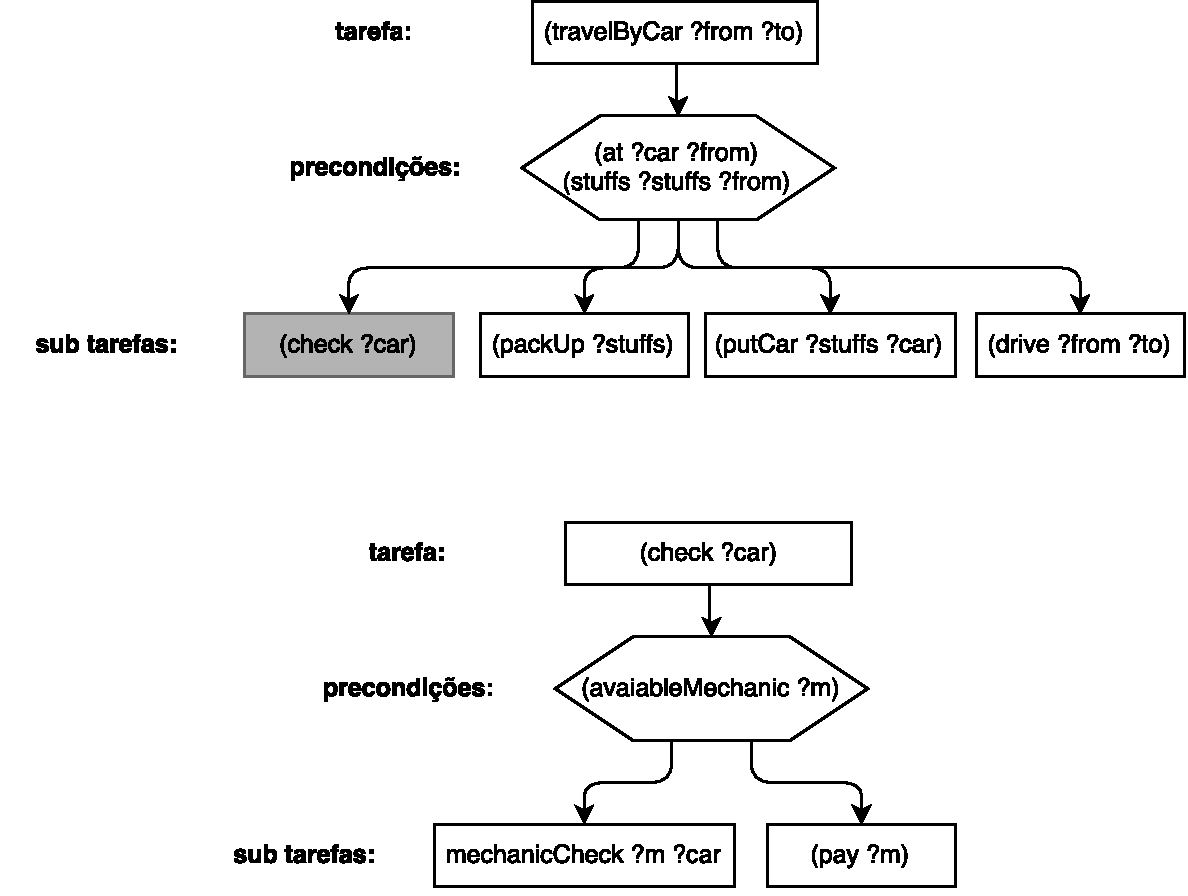
\includegraphics[width=0.7\textwidth]{fig/htnmethod.pdf}
	\caption{Exemplo de método HTN.}
	\label{fig:htnmethod}
\end{figure} 

Um problema de planejamento HTN $P$ é definido como $P = (d, I, D)$, onde $D$ é um domínio, $d$ é a tarefa de ligação inicial e $I$ é um estado inicial como no planejamento clássico. 
O processo de geração de um plano utilizando planejamento HTN consistem em encontrar um método que consiga ser aplicado na primeira tarefa de $d$, isso faz com que seja gerado uma tarefa de ligação diferente $d'$, onde a primeira tarefa foi decomposta. 
Esse processo continua, agora aplicado a $d'$, até que todas as tarefas sejam primitivas \cite{meneguzzi2015planning}. 
Se em algum ponto, nenhum método consiga ser aplicado, o planejador deve realizar um retrocesso(\textit{backtracking}), que consiste em voltar a um $d$ anterior a ponto de conseguir aplicar outra decomposição \cite[Capítulo 11]{intelligence2003modern}. 
É possível representar a busca do plano por uma árvore $N$, na qual os nodos são tarefas ou métodos. 
Cada tarefa não-primitiva pode ter apenas um filho, que deve ser um método. 
Cada método deve ter um filho para cada uma das suas sub tarefas. 
Tarefas primitivas não podem ter filhos, o que significa que elas não podem ser decompostas. 
Uma árvore totalmente decomposta, é onde todas as folhas de $N$ são tarefas primitivas \cite{ontanon2015adversarial}. 
A Figura~\ref{fig:htnmethodtree} ilustra a árvore de resolução do exemplo anterior.

\begin{figure}[ht]
	\centering
	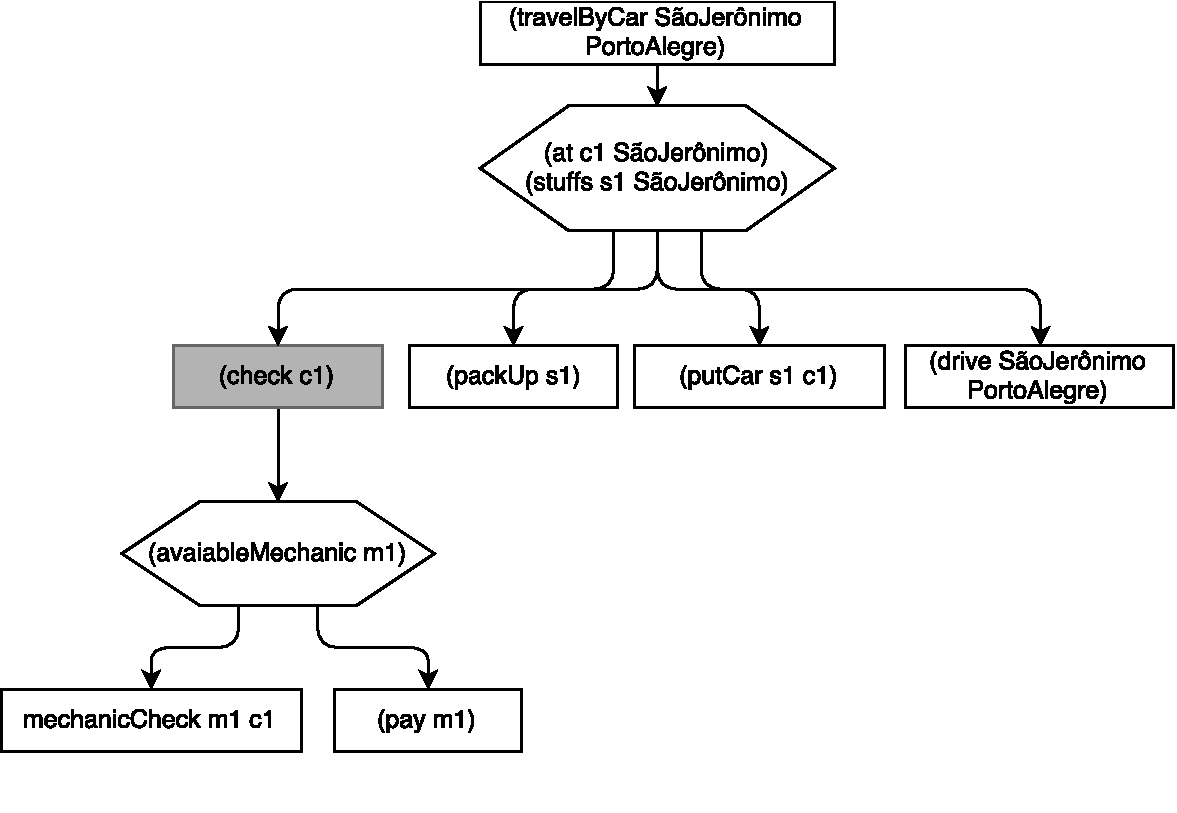
\includegraphics[width=0.7\textwidth]{fig/htnmethodresult.pdf}
	\caption{Arvore de resolução HTN.}
	\label{fig:htnmethodtree}
\end{figure}

O algoritmo de \textit{Total-order Forward Decomposition} (TFD) é utilizado para gerar um plano a partir de uma rede de tarefas inicial com ordenação total, como detalhado no Algoritmo~\ref{alg:tfd}.
O algoritmo gera as ações na mesma ordem que serão executadas, então a cada vez que uma tarefa é alcançada, tudo que antecede a mesma já foi planejado \cite{ghallab2004automated}.
 
\begin{algorithm}
	\caption{Total-order Forward Decomposition}
	\label{alg:tfd}
	\begin{algorithmic}[1]		
		\Function {TFD}{$s, <t_{1}, ...,t_{k}>, O, M$}
			\If {$k = 0$}
				\State	\Return $<>$
			\EndIf
			\If {$t_{1}$ é primitivo}
				\State $ativo = \{(a, b)~ |$ $a$ é uma instancia de $O$ e é aplicável a $s$ e b é uma substituição que torna $a$ relevante para $b(t_{1})\}$
				\If {$ativo = \emptyset$}
					\State \Return falha
				\EndIf
				\State escolhe algum par $(a, b) \in active$
				\State $\pi = TFD(\gamma(s, a), b(<t_{2}, ..., t_{k}>, O, M)$
				\If {$\pi = falha$}
					\State \Return falha
				\Else 
					\State \Return $a . \pi$
			\EndIf
			
			\ElsIf {$t_{1}$ é não primitiva}
				\State $ativo = \{m |~ m$ é aplicável a $s$ e $m \in M\}$
				\If {$ativo = \emptyset$}
					\State \Return falha
				\EndIf
				\State escolhe algum par $(m, b) \in active$
				\State $w =~ $subtarefas$(m).b(<t_{2}, ..., t_{k}>)$
				\State \Return $TFD(s, w, O, M)$
				\EndIf
		\EndFunction
	\end{algorithmic}
\end{algorithm}

\section{Adversarial hierarchical-task network} \label{sec:ahtn}

\textit{Adversarial hierarchical-task network} (AHTN) é um algoritmo desenvolvido para lidar com o problema do grande fator de ramificação dos jogos em tempo real~\cite{ontanon2015adversarial} utilizando conhecimento de domínio no estilo de planejamento HTN. 
Nele são combinados técnicas de HTN com o algoritmo \textit{minimax search}. 
O algoritmo assume jogos totalmente observáveis, baseados em turno e determinísticos. 

O Algoritmo~\ref{alg:ahtn}~\cite{ontanon2015adversarial} é a representação da técnica de AHTN, e assume que existem dois jogadores, \textsc{Max} e \textsc{Min}, como no algoritmo de \textit{minimax search} apresentado na Seção~\ref{sec:minimax}. 
O algoritmo também assume uma busca em uma árvore com uma máxima profundidade $d$. 
O intuito do algoritmo de AHTN é gerar os melhores plano para \textsc{Max} e para \text{Min}, junto com o resultado de uma função de avaliação para quando os planos chegam a um estado terminal. 

\begin{algorithm}
	\caption{Adversarial hierarchical-task network}
	\label{alg:ahtn}
	\begin{algorithmic}[1]		
		\Function {AHTNMax}{$s, N_{+}, N_{-}, t_{+}, t_{-}, d$}
		\If {$terminal(s) \vee d \leq 0$}\label{alg:lin:firstLine}
		\State	\Return $(N_{+}, N_{-}, e(s))$
		\EndIf
		\If {$nextAction(N_{+}, t_{+}) \neq \perp$} \label{alg:ahtn:nexaction}
		\State $t = nextAction(N_{+}, t_{+})$ 
		\State \Return $\Call{AHTNMin}{(\gamma(s,t), N_{+}, N_{-}, t, t_{-}, d-1)}$ \label{alg:ahtn:troca}
		\EndIf
		\State $N_{+}^{*} = \perp, N_{-}^{*} = \perp, v^{*} = -\infty$
		\State $\aleph = decompositions_{+}(s, N_{+}, N_{-}, t_{+}, t_{-})$ \label{alg:decompositions}
		\ForAll{$N \in \aleph$} \label{alg:ahtn:for}
		\State $(N^{'}_{+}, N^{'}_{-}, v^{'}) = AHTNMax(s, N, N_{-}, t_{+}, t_{-}, d)$
		\If{$v^{'} > v^{*}$}
		\State $N_{+}^{*} = N^{'}_{+}, N_{-}^{*} = N^{'}_{-}, v^{*} = v^{'} $
		\EndIf
		\EndFor		
		\State \Return $(N_{+}^{*}, N_{-}^{*}, v^{*} )$
		\EndFunction
	\end{algorithmic}
\end{algorithm}

O algoritmo de AHTN gera uma árvore das jogadas. Cada nodo da árvore é definido por uma tupla $(s, N_{+}, N_{-}, t_{+}, t_{-})$, onde $s$ é o estado corrente do ambiente, $N_{+}$ e $N_{-}$ são a representação de planos HTN para os jogadores \textsc{Max} e \textsc{Min}, respectivamente, $t_{+}$ e $t_{-}$ representam ponteiros para qual parte do plano HTN está sendo executada, sendo $t_{+}$ para uma tarefa de $N_{+}$ e $t_{-}$ para uma tarefa de $N_{-}$. Cada nodo da árvore representa um estado do jogo~\cite{ontanon2015adversarial}.

O algoritmo alterna a perspectiva dos jogadores sempre que existir uma tarefa primitiva no plano atual, e assim avança na profundidade da árvore das jogadas. A função $AHTNMin$ é responsável pela mudança de perspectiva, e ela está presente no bloco que inicia na Linha~\ref{alg:ahtn:nexaction}. No mesmo bloco há a função \texttt{nextAction(N,t)}, que é responsável por verificar é possível a troca de perspectiva. Ela recebe como parâmetro um plano ($N$) e um ponteiro ($t$). Com isso ela retorna um ponteiro para a próxima tarefa primitiva, caso ainda não haja uma tarefa primitiva no plano, a função retorna $t = \bot$.

Caso não seja possível trocar de perspectiva, o algoritmo de AHTN decompõe o plano. O método $decompositions$ é responsável por decompor o plano atual a partir do estado do jogo na árvore. O método apenas adiciona novos planos que utilizem apenas um novo método ao plano atual. A chamada deste método ocorre na Linha~\ref{alg:decompositions} do algoritmo gerando novos planos.
O algoritmo utiliza as decomposições para comparar todos os planos gerados por uma função de avaliação. O plano que tiver a melhor função de avaliação é escolhido como melhor caminho. O plano escolhido é retornado junto com o resultado da função de avaliação. Este processo está presente na Linha~\ref{alg:ahtn:for}.

O plano pode acabar quando a profundidade limite for atingida, ou quando um estado terminal for alcançado.
Quando alguma dessas condições for alcançada, é retornado o plano das duas perspectivas e a função de avaliação para o estado do jogo atual. A Linha~\ref{alg:lin:firstLine} mostra essa condição.

A grande diferença entre o algoritmo de $AHTN$ e o algoritmo do \textit{minimax search}, é que as chamadas recursivas nem sempre se alternam entre \textsc{Max} e \textsc{Min}. 
O algoritmo troca de nodos \textsc{Max} para \textsc{Min} apenas quando os planos estão totalmente decompostos a ponto de gerar uma ação (Linha \ref{alg:ahtn:troca})~\cite{ontanon2015adversarial}.

A Figura~\ref{fig:ahtn}\footnote{Figura extraída de~\cite{ontanon2015adversarial}} é utilizada para exemplificar o funcionamento do algoritmo~\ref{alg:ahtn}. 
Na raiz da árvore há apenas uma tarefa não primitiva \textit{win} para ser decomposta, para os dois jogadores. 
Há duas decomposições que o jogador \textsc{Max} pode aplicar para seu plano HTN, resultando nos nodos $n_{1}$ e $n_{5}$. A decomposição $n_{1}$ não resulta em nenhuma ação primitiva, e por isso $n_{1}$ continua um nodo \textsc{Max}. Uma vez que o jogador \textsc{Max} decompõe seus planos e há tarefas primitivas para serem executadas (nodos $n_{2}$ e $n_{5}$), é o turno de \textsc{Min} decompor suas tarefas não primitivas. Após \textsc{Min} gerar suas ações, a profundidade máxima ($d = 2$) foi atingida (nodos $n_{3}$ e $n_{4}$). 
A função de avaliação $e$ é aplicada para cada um dos estados do jogo para determina o valor das folhas.

\begin{figure}[ht]
	\centering
	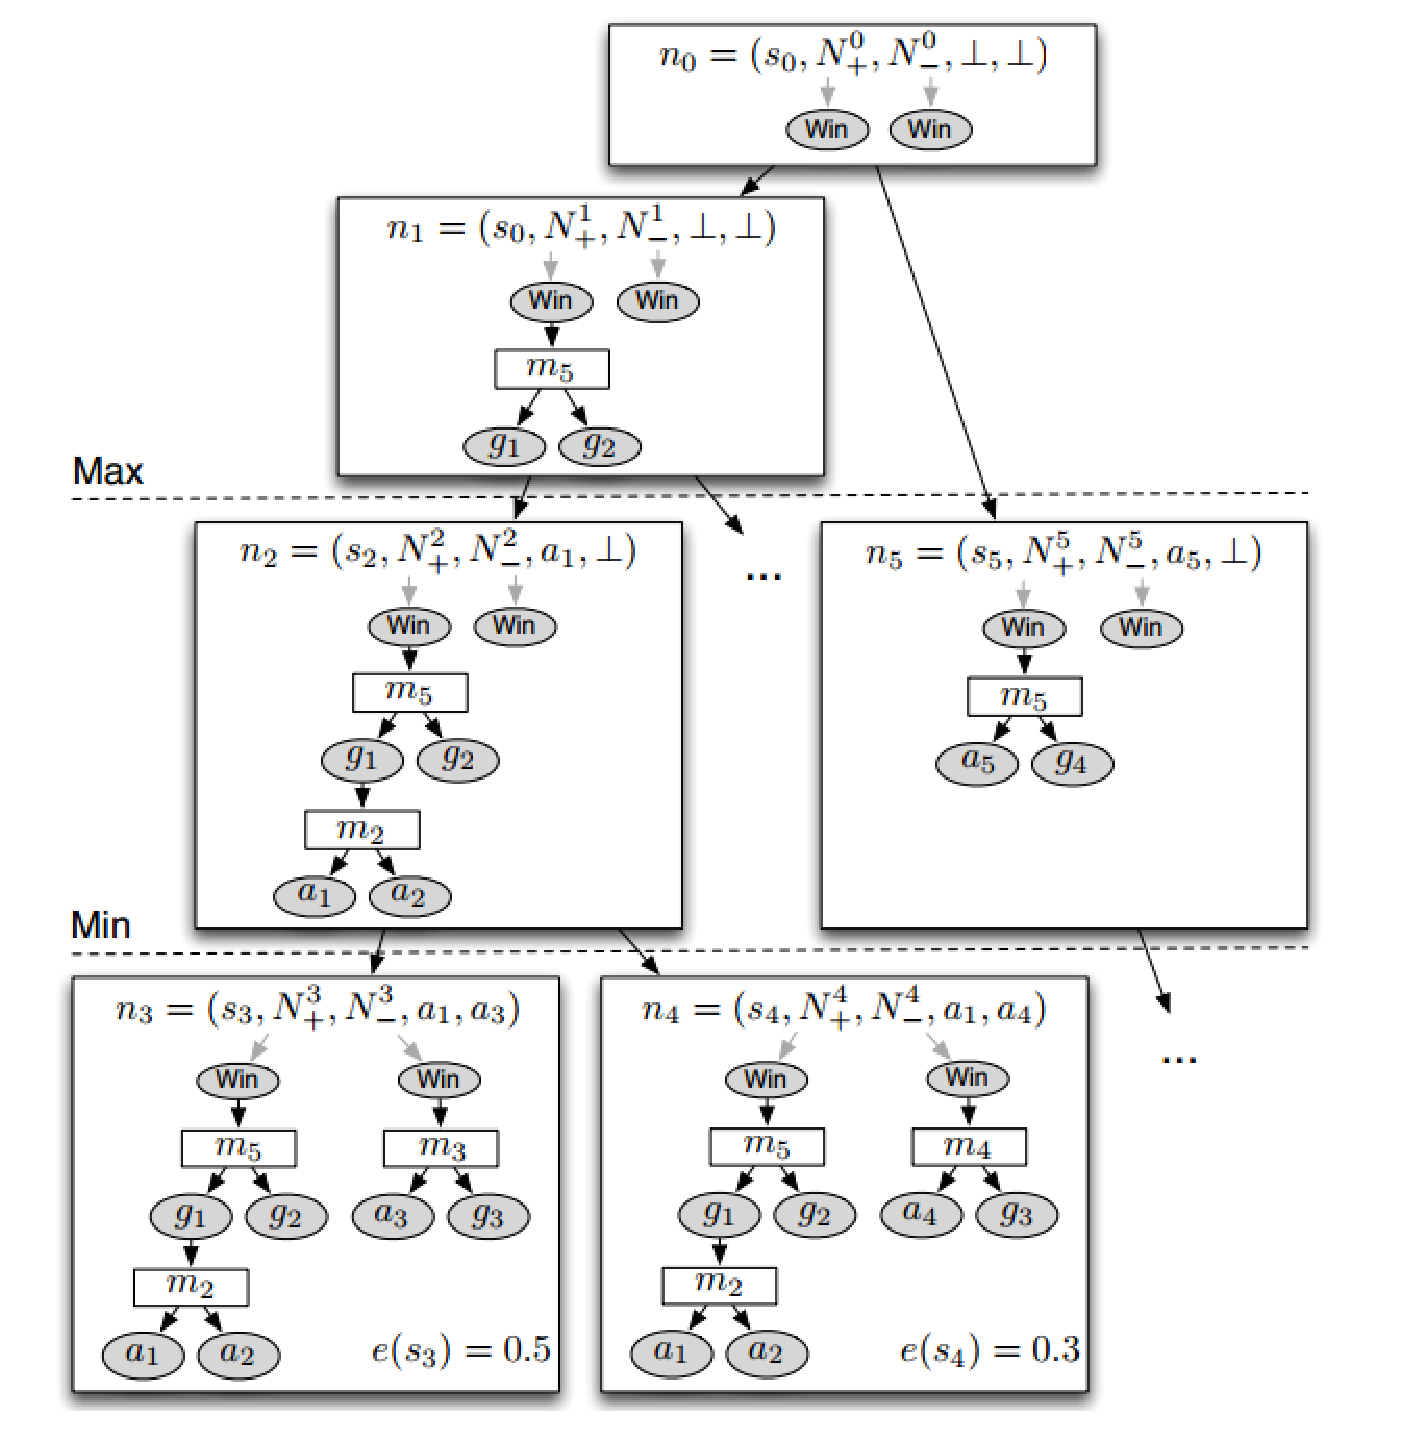
\includegraphics[width=0.8\textwidth]{fig/ahtn.pdf} 
	\caption{Árvore gerada pelo algoritmo de AHTN.}
	\label{fig:ahtn}
\end{figure}

O problema que o algoritmo de AHTN tenta lidar é o grande fator de ramificação e o pouco tempo para determinar a próxima ação do agente. O algoritmo utiliza planejamento através do conhecimento de domínio para diminuir a combinação de ações que não tem nenhuma chance de ser usadas em um jogo real~\cite{ontanon2015adversarial}. 

%!TEX root = volumeFinal.tex 
\chapter{\label{chap:aprendizado}Aprendizado}
 
Para os humanos o aprendizado ocorre durante toda a vida. 
O aprendizado é o ato de adquirir novos conhecimentos, ou modificar conhecimentos já existentes ou ainda adquirir uma experiência por repetição do ato de forma incorreta. 
Aprendizado pode variar de adquirir conhecimento de tarefas simples, como decorando um número de telefone, até tarefas mais complicadas, como a formulação de novas teorias \cite{intelligence2003modern}. 

\section{Aprendizado de Máquina} 

A área na computação que estudo esse aprendizado de forma computacional é o aprendizado de máquina, melhor conhecida como \textit{machine learning}. 
A definição de aprendizado de máquina proposta por Tom Mitchell \cite{Mitchell1997ML} é a seguinte:

\begin{quote}
	Definição: Um programa de computador é dito que aprende de uma experiência E com relação a alguma classe de tarefas T, e medida de performance P, se essa performance sobre as tarefas em T, medida por P, melhora com a experiência E.
\end{quote}

Essa definição mostra que o sistema aprimora seu conjunto de tarefas T com uma performance P através de experiências E. 
Ou seja, um sistema baseado em aprendizado de máquina deve, através de experiências, ter um ganho nas informações para solucionar os seus problemas. 
Para começar a resolver um problema utilizando aprendizado de máquina é preciso escolher qual experiência será aprendida pelo sistema \cite{Mitchell1997ML}. 
Para isso existem algumas técnicas que tratam aprendizado de máquina com objetivos diferentes \cite{intelligence2003modern}. 
Alguma das técnicas são: 
\begin{itemize}
	\item aprendizado supervisionado: que consiste em aprender através de algum conjunto de exemplos a realizar a classificação de algum problema. Cada problema é mapeado para uma saída;  
	\item aprendizado não supervisionado: que consistem em aprender através das observações, algum padrão ou regularidade, para classificar em grupos os problemas; e 
	\item aprendizado por reforço: que consiste em aprender, através das execuções de um agente, quais ações possuem maior recompensa média esperada.
\end{itemize}

Cada tipo de aprendizado é utilizado pode ser usado para uma aplicação especifica, mas existem casos em que a combinação das técnicas se mostra mais eficaz. 
Um exemplo apresentado por \cite{intelligence2003modern} é o reconhecimento de idade por fotos, para essa tarefa são necessários amostras de fotos com as idades, então a técnica que se encaixa é aprendizado supervisionado, mas existem ruídos aleatórios nas imagens que fazem com que a precisão da abordagem caia, para superar esse problema pode ser combinado aprendizado supervisionado com o não supervisionado.

\section{Aprendizado por Reforço}

O aprendizado por reforço também é conhecido como \textit{reinforcement learning}. Este tipo de aprendizado utiliza \textit{feedbacks}, vindas do ambiente após a sua execução, esse tipo de \textit{feedback}, é chamado de recompensa. O objetivo deste aprendizado é usar as recompensas obtidas nas observações para aprender uma política do ambiente ou determinar o quão boa a política é \cite{intelligence2003modern}. 

Em jogos \textit{reinforcement learning} é um tópico que é bastante utilizado \cite{millington2009artificial}. Em um jogo essa técnica utiliza três etapas, uma para exploração da estratégia para achar as diferentes ações possíveis no jogo, uma função que disponibiliza o \textit{feedback} e diz o quão bom é cada ação, e uma regra de aprendizado que junta as outras duas etapas \cite{millington2009artificial}.

Existem dois tipos principais de aprendizado por reforço \cite{intelligence2003modern}: aprendizado passivo, e aprendizado ativo; detalhados nas seções a seguir. 

\subsection{Aprendizado passivo} 

O aprendizado passivo utiliza ambientes completamente observáveis. A política do agente $\pi$ é fixa, em um estado $s$, sempre é executado a mesma ação $\pi(s)$. O objetivo desse tipo de aprendizado é aprender o quão bom é a política, o que significa aprender a função de utilidade $U^{\pi}(s)$. Um agente que utiliza aprendizado passivo não conhece o modelo de transição $P(s' | s, a)$, que especifica a probabilidade de alcançar o estado $s'$ a partir do estado $s$ executando a ação $a$, e também não conhece a função de recompensa $R(s)$, que especifica a recompensa de cada estado \cite{intelligence2003modern}. 

Um agente que utiliza essa técnica realiza várias execuções do ambiente utilizando a politica $\pi$. Em cada tentativa o agente inicia no mesmo estado inicial e realiza uma sequência de transições de estados até chegar a um estado terminal. As percepções obtidas com essas execuções, em cada estado, servem para descobrir a recompensa obtida nos estados. O objetivo é utilizar a informação das recompensas para aprender a utilidade esperada $U^{\pi}(s)$ associada a cada estado $s$ não terminal \cite{intelligence2003modern}. 

\subsection{Aprendizado ativo}

O aprendizado ativo diferente do passivo não tem uma política fixa e a mesma deve ser aprendida. Para isso, um agente que utiliza este tipo de aprendizado precisa decidir quais ações tomar, isso faz com que o agente precise aprender o modelo de transição $P(s' | s, a)$ para cada um dos estados e ações \cite{intelligence2003modern}. 

Um método para conseguir definir a política do ambiente é chamado de \textit{Q-learning}. O objetivo desse método é aprender uma utilidade ligada a um par de estado e ação, a notação $Q(s, a)$, representa o valor de executar a ação $a$ no estado $s$. Este método está relacionado com o valor de utilidade presente na equação \ref{eq:qler} \cite{intelligence2003modern}.

\begin{equation}
\label{eq:qler}	
	U(s) =  max_{a} Q(s, a)
\end{equation}

O algoritmo de \textit{Q-learning} não precisa aprender o modelo de transição $P(s' | s, a)$, por esse motivo ele é chamado de um método livre de modelo. A equação \ref{eq:qler2} representa o cálculo do valor de $Q(s, a)$.

\begin{equation}
\label{eq:qler2}	
Q(s, a) = Q(s, a) + \alpha (R(s) + \gamma max_{a'} Q(s', a') - Q(s, a))
\end{equation}

O valor $\alpha$ representa a taxa de aprendizado do agente, variando de 0 a 1, nele é contido a informação se o agente deve considerar as informações obtidas em um novo aprendizado ou não, sendo 1 se considera inteiramente o que foi aprendido, e 0 se for descartar as novas informações. $R(s)$ é a recompensa obtida ao alcançar o estado $s$. O valor de $\gamma$ representa o fator de desconto, que descreve a preferência do agente em receber recompensas futuras ou recompensas locais, o seu valor varia entre 0 e 1, quando 0 apenas as recompensas locais são utilizadas, e quando 1 as recompensas futuras são totalmente utilizadas. O Algoritmo~\ref{alg:qlearning} ilustra o método de \textit{Q-learning} para um agente \cite{intelligence2003modern}. A Linha~\ref{alg:qlearning:form} é onde é atualizado o valor de $Q(s, a)$ utilizando a Formula~\ref{eq:qler2}. O algoritmo leva em conta quantas vezes quantas vezes o valor $Q(s, a)$ foi calculado, incrementando a cada nova passada do algoritmo pela Linha~\ref{alg:qlearning:increment}. O algoritmo indica a melhor ação para o estado atual.  

\begin{algorithm}
	\caption{Q-Learning}
	\label{alg:qlearning}
	\begin{algorithmic}[]	
		\Function{Q-Learning}{$state, reward$}
		\If {$terminal(state)$}
		\State	\Return $Q[s, None] = reward$
		\EndIf
		\If {$state$ is not null}
		\State {increment $N[s, a]$} \label{alg:qlearning:increment}
		\State $Q[s, a] = Q[s, a] + \alpha(N[s, a]) (r + \gamma max_{a'} Q[s', a'] - Q[s, a])$ \label{alg:qlearning:form}
		\State $s = s'$
		\State $a = argmax_{a'} f(Q[s', a'], N[s', a'])$ \label{alg:qlearning:f}
		\State $r = r'$
		\EndIf	
		\State \Return $a$
		\EndFunction
	\end{algorithmic}
\end{algorithm}

\frm[inline]{Acho que vale a pena colocar um pouquinho mais aqui, tipo SARSA e a generalização.}

As técnicas de aprendizado de máquina têm grande potencial na área de jogos. O aprendizado de máquina consegue que os agentes reproduzam jogadores mais interessante, pelo fato de que os agentes aprendem sobre o ambiente e usam essa informação a seu favor em jogadas futuras. Os agentes aprendem táticas de jogos com suas derrotas e as aperfeiçoam com suas vitorias. Utilizar técnicas de aprendizado de máquina exige um cuidado e um entendimento das necessidades do jogo \cite{millington2009artificial}. O intuito de adicionar um algoritmo de aprendizado de máquina ao trabalho, vem do fato de que com as informações, provenientes das observações, é possível acrescentar um conhecimento extra nas próximas execuções, a fim de não cometer os mesmos erros de observações anteriores. \frm[color=yellow]{Tu tens que fechar o capítulo de alguma forma, e dizer por que isto está aqui. No projeto tu também tens que referenciar este capítulo.}

%%!TEX root = volumeFinal.tex 
\chapter{\label{chap:games}Jogos}
 
  Jogos eletrônicos são muito populares, principalmente pela grande quantidade de gêneros, existem jogos de ação, aventura, esportes, estrategia, entre outros. Hoje em dia, os jogos buscam que quem jogue consiga ficar imerso no dentro do jogo, sem conseguir identificar um padrão nos jogadores fictícios, pois se não o jogo deixa de ser tão interessante. Para que isso aconteça, a IA é associada a diversos jogos, e é comum pensar que quanto mais complexa a IA aplicada dentro do jogo mais difícil jogo irá ficar, mas isso nem sempre é verdade, nem sempre IA complicadas terão melhor desempenho do que as mais simples, uma boa IA dentro do jogo é feita a partir de determinar o comportamento certo para os algoritmo certos \cite{millington2009artificial}.
  
 \section{Jogos de estratégia em tempo real}
 
Jogos de estratégia em tempo real, também conhecido por \textit{real-time strategy games} (RTS), é um sub-gênero de jogos de estrategia, onde os jogadores precisam construir uma base com uma economia, ganhando recursos, construindo edificações, treinando unidades de ataques e tecnologias para elas, tudo isso com o objetivo de destruir uma ou mais bases inimigas \cite{ontanon2013survey, buro2012real}. 

Existem algumas diferenças entre jogos RTS e jogos de tabuleiro, como xadrez. Estas diferenças são \cite{ontanon2013survey}:

\begin{itemize}
	\item Movimentos simultâneos- jogadores realizam jogadas ao mesmo tempo;
	\item Tempo real- cada jogador deve realizar suas ações em um curto espaço de tempo;
	\item Parcialmente observável- na maioria dos jogos RTS, o jogador só consegue enxergar parte do ambiente;
	\item Não-determinístico- nem sempre uma ação realizada resulta  na saída esperada;
	\item Complexidade- O espaço de estados e o número de ações possíveis é muito grande.
\end{itemize} 


Pelo fato de existirem essas diferenças, não é possível traduzir automaticamente as técnicas padrões dos jogos de tabuleiro para jogos RTS sem algum tipo de abstração ou simplificação \cite{ontanon2013survey}.
 
\subsection{MicroRTS}  
 
Um exemplo deste gênero é o Starcraft\footnote{http://us.battle.net/sc2/pt/}. Uma simplificação do Starcraft foi feita por Santiago Ontañón \cite{ontanon2013combinatorial}, chamada de MicroRTS. O MicroRTS foi desenvolvido para fins acadêmicos, com o intuito de aplicar e desenvolver técnicas de IA e para servir como prova de conceito para as técnicas criadas.

\todo[inline]{como o jogo funciona?} 
O objetivo do jogo é destruir a base adversaria. Existem trabalhadores que podem coletar recursos e construir outros prédios. Os recursos são coletados dos minerais. Com os recursos é possível construir bases de ataque, onde são realizado o treinamento de unidades de ataque. Para conseguir realizar o objetivo de destruir a base adversaria é preciso ter unidades de ataque. O jogo oferece três destas unidades, são elas:
 
 \begin{itemize}
 	\item Heavy - Possui um alto poder de ataque, mas sua velocidade é lenta.
 	\item Light - Possui um baixo poder de ataque, mas sua velocidade é rápida.
 	\item Ranged - Possui um ataque de longa distancia. 
 \end{itemize} 
 
 A Figura~\ref{fig:microrts}\footnote{https://github.com/santiontanon/microrts} mostra uma tela do jogo que representa o que foi explicado e ainda é possível observar que o fator de ramificação pode ser muito alto dependendo do cenário do jogo.
 
 \begin{figure}[ht]
 	\centering
 	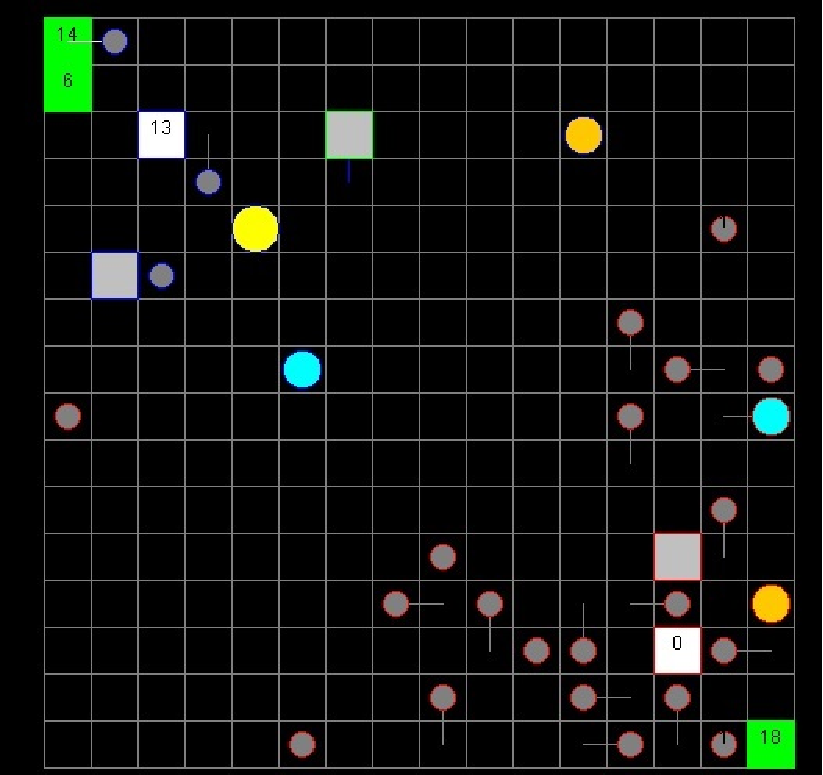
\includegraphics[width=0.5\textwidth]{fig/microrts.pdf}
 	\caption{Um exemplo de tela do MicroRTS}
 	\label{fig:microrts}
 \end{figure} 
 
\todo[inline]{abordagens já implementadas} 
No ambiente há algumas estrategias implementadas, cada estrategia possui variações dos algoritmos. Algumas das estrategias são:
 \begin{itemize}
 	\item Minimax Alpha-Beta Search Strategies - O que muda entre as técnicas é o jeito com que é feito a expansão do grafo.
 	\item Monte Carlo Search Strategies - Executa jogadas aleatórias para planejar e após utiliza uma heurística para determinar em qual caminho seguir.
 \end{itemize}
 
A plataforma já foi utilizada para aplicar técnica de IA. Por esse motivo a utilização dela se torna viável para a realização deste trabalho. 
 
 
 
 
%!TEX root = proposta.tex 
\chapter{\label{chap:obje}Objetivos}

Atualmente, há uma dificuldade na utilização de técnicas de IA para jogos em tempo real. Isso ocorre pelo fato que a IA precisa ser capaz de resolver tarefas, do mundo real, de maneira rápida e satisfatória. Geralmente, o espaço de estados dos jogos é enorme, isso faz com que não se tenha tempo de explorar todas as possibilidades de solução.   \\

%\frm{Seja mais específico, o que é difícil? Faltam técnicas?}

O intuito desse trabalho é mostrar que uma abordagem híbrida com planejamento e aprendizado de maquina pode ser uma alternativa valida para tratar esse gênero de jogo. 
%\frm{Não é bem a leitura de livros, tu vais te basear em um algoritmo específico que tu encontraste}
A leitura de livros será utilizada para adquirir embasamento teórico \cite{ghallab2004automated,intelligence2003modern,Mitchell1997ML} para entender as técnicas utilizadas no algoritmo AHTN \cite{ontanon2015adversarial}. Já a leitura dos artigos ajudará com a análise dos resultados \cite{ontanon2012experiments,hogg2010learning,ontanon2013survey}.
 \\ 
O jogo escolhido como plataforma foi o MicroRTS \cite{ontanon2013combinatorial}, pelo fato de que o jogo é uma simplificação de um jogo em tempo real, e é utilizado para demonstrar outras técnicas de IA . Como o jogo escolhido como plataforma já tem alguns algoritmos de IA implementados %\frm{Tu estás mencionando o jogo o qual tu ainda nem falou!!}
, a comparação com outros algoritmos pode ser considerado algo mais simples. %
%\frm{Talvez mover os objetivos para depois?} 

%\section{Objetivo Geral}

%O objetivo geral deste trabalho é implementar o algoritmo de planejamento AHTN \cite{ontanon2015adversarial} que combina técnicas de HTN com o algoritmo de \textit{minimax serach}. Após implementado, integrar aprendizado por reforço através da ferramenta WEKA\footnote{http://www.cs.waikato.ac.nz/ml/weka/} com o objetivo de melhorar o desempenho do algoritmo. Ao final do trabalho, o objetivo é conseguir comparar resultados obtidos com os resultados já publicados e consolidados \cite{ontanon2007case,ontanon2012experiments,hogg2010learning,buro2003real,ontanon2013survey}.  

\section{Objetivos Específicos}
\label{obj:esp}
\begin{itemize}
\item Estudar algoritmos de HTN.
\item Estudar o algoritmo de AHTN.
\item Estudar algoritmos de aprendizado por reforço.
\item Estudar como unir o algoritmo de AHTN com uma técnica de aprendizado por reforço. %\frm{E o AHTN? Te lembra que usamos aprendizado de máquina em minimax para compensar a falta de tempo para explorar tudo.}
\item Avaliar a aplicabilidade desses algoritmos junto ao jogo escolhido.
\item Definir a estratégia de implementação do algoritmo escolhido.
\item Comparar resultados com outras abordagens.
\end{itemize}



%\frm[inline]{De repente remover este objetivo}
%\section{Objetivo Adicional}

%Caso for possível atingir todos os objetivos propostos na seção \ref{obj:esp}, existe um item adicional %para aplicar a este trabalho:

%\begin{itemize}
%\item Testar o algoritmo em outro jogo RTS, como por exemplo Battle for Wesnoth\footnote{https://www.wesnoth.org/}\frm{Wesnoth não é RTS é um jogo de estratégia por turnos}.
%\end{itemize}

%!TEX root = volumeFinal.tex 
\chapter{\label{chap:ativ}Análise e Projeto}

\section{Jogos}
 Jogos eletrônicos são muito populares, principalmente pela grande quantidade de gêneros, existem jogos de ação, aventura, esportes, estratégia, entre outros. Hoje em dia, os jogos buscam que quem jogue consiga ficar imerso no dentro do jogo, sem conseguir identificar um padrão nos jogadores fictícios, pois se não o jogo deixa de ser tão interessante. Para que isso aconteça, a IA é associada a diversos jogos, e é comum pensar que quanto mais complexa a IA aplicada dentro do jogo mais difícil jogo irá ficar, mas isso nem sempre é verdade, nem sempre IA complicadas terão melhor desempenho do que as mais simples, uma boa IA dentro do jogo é feita a partir de determinar o comportamento certo para os algoritmo certos \cite{millington2009artificial}.
 
 \subsection{Jogos de estratégia em tempo real}
 
 Jogos de estratégia em tempo real, também conhecido por \textit{real-time strategy games} (RTS), é um subgênero de jogos de estratégia, onde os jogadores precisam construir uma base com uma economia, ganhando recursos, construindo edificações, treinando unidades de ataques e tecnologias para elas, tudo isso com o objetivo de destruir uma ou mais bases inimigas \cite{ontanon2013survey, buro2012real}. 
 
 Existem algumas diferenças entre jogos RTS e jogos de tabuleiro, como xadrez. Estas diferenças são \cite{ontanon2013survey}:
 
 \begin{itemize}
 	\item movimentos simultâneos, jogadores realizam jogadas ao mesmo tempo;
 	\item tempo real, cada jogador deve realizar suas ações em um curto espaço de tempo;
 	\item parcialmente observável, na maioria dos jogos RTS, o jogador só consegue enxergar parte do ambiente;
 	\item não-determinístico, nem sempre uma ação realizada resulta na saída esperada; e
 	\item complexidade, O espaço de estados e o número de ações possíveis é muito grande.
 \end{itemize} 
 
 
 Pelo fato de existirem essas diferenças, não é possível traduzir automaticamente as técnicas padrões dos jogos de tabuleiro para jogos RTS sem algum tipo de abstração ou simplificação \cite{ontanon2013survey}.
 
\subsection{MicroRTS}  
 
 Um exemplo deste gênero é o MicroRTS\footnote{https://github.com/santiontanon/microrts}, uma simplificação do jogo Starcraft\footnote{http://us.battle.net/sc2/pt/}, feita por Santiago Ontañón \cite{ontanon2013combinatorial} em Java. O MicroRTS foi desenvolvido para fins acadêmicos, com o intuito de aplicar e desenvolver técnicas de IA e para servir como prova de conceito para as técnicas criadas.
 
 \begin{figure}[ht]
 	\centering
 	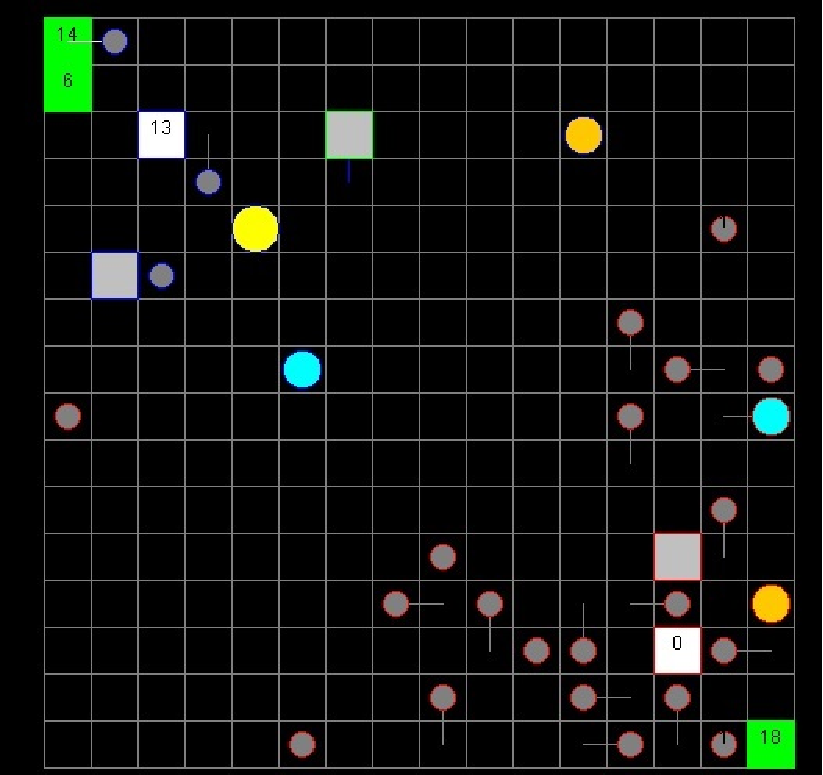
\includegraphics[width=0.5\textwidth]{fig/microrts.pdf}
 	\caption{Um exemplo de tela do MicroRTS}
 	\label{fig:microrts}
 \end{figure} 
 
O MicroRTS consiste em dois jogadores tentando destruir a base adversaria. Para destruir com o inimigo é preciso eliminar cada unidade e edificações adversarias. A Figura~\ref{fig:microrts} mostra uma tela do jogo. Existem quatro tipos de unidades no jogo, são elas:
  
\begin{itemize}
 	\item \textit{worker}, é responsável por coletar recursos e construir as edificações. Esta unidade também consegue lutar, mas possui um dano muito baixo;
 	\item \textit{heavy}, unidade que pode apenas atacar. Ela possui um alto poder de ataque, mas sua velocidade é lenta;
 	\item \textit{light}, unidade que pode apenas atacar. Ela possui um baixo poder de ataque, mas sua velocidade é rápida; e
 	\item \textit{ranged}, unidade que pode apenas atacar. Ela possui um ataque de longa distância. 
\end{itemize} 
 
Para adquirir as unidades é preciso das edificações e recursos. Existem três tipos de edificações, são elas:

\begin{itemize}
	\item base, a base é a edificação principal, ela é responsável pela criação dos \textit{workers}, e nela também é guardado os recursos coletados pelos \textit{workers};
	\item quartel, o quartel é responsável pela criação das unidades de ataque \textit{heavy}, \textit{light} e \textit{ranged}. Ela pode ser construída pelos \textit{workers} usando recursos; e
	\item base de recurso, na base de recurso são coletados os recursos pelos \textit{workers}, os a base de recursos é finitos para ser coletada.
\end{itemize}  

No início do jogo, cada jogador inicia com uma base, um \textit{worker} e uma base de recurso para coletar. Todas as unidades podem ser atacas menos a base de recursos. 
 
No ambiente há algumas estratégias implementadas, cada estratégia possui variações dos algoritmos. Algumas das estratégias são:
 \begin{itemize}
 	\item \textit{Minimax Alpha-Beta Search Strategies} - O que muda entre as técnicas é o jeito com que é feito a expansão do grafo.
 	\item \textit{Monte Carlo Search Strategies} - Executa jogadas aleatórias para planejar e após utiliza uma heurística para determinar em qual caminho seguir.
 \end{itemize}
 
 A plataforma já foi utilizada para aplicar técnica de IA. Por esse motivo a utilização dela se torna viável para a realização deste trabalho. 
Nela é possível observar que o fator de ramificação pode ser muito alto dependendo do cenário do jogo.

\subsection{Arquitetura do MicroRTS}

A arquitetura do MicroRTS é composta por 4 componentes principais: O Jogo em si, onde são feitas todas as ações dos jogos. As unidades, onde todas as ações de cada unidade podem ser controladas e acessadas, por exemplo, saber onde está cada unidade inimiga. A Interface gráfica, responsável pela representação gráfica do jogo. E a Inteligência Artificial, onde pode ser acoplado a IA que desejar, a plataforma já possui algumas como foi dito anteriormente. A imagem \ref{fig:pacotes} representa os componentes.

 \begin{figure}[ht]
 	\centering
 	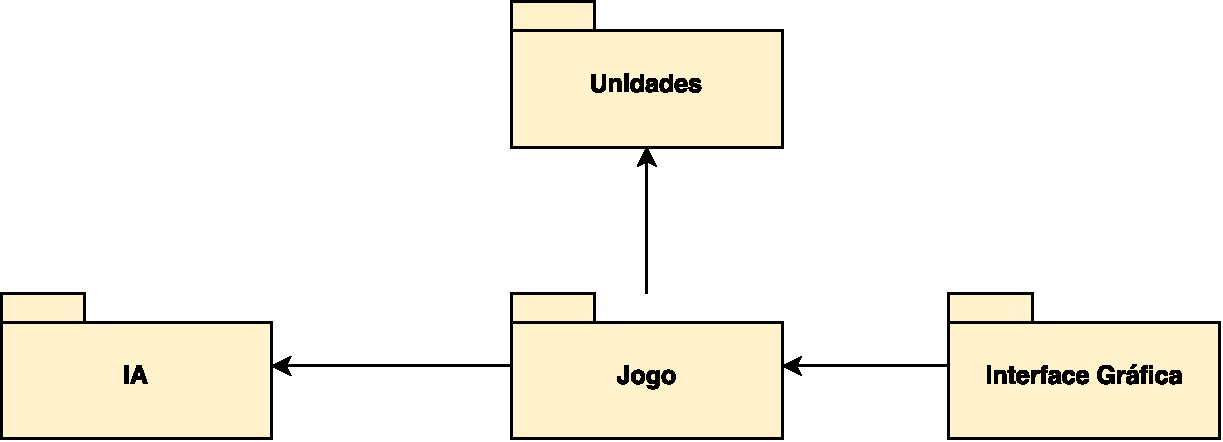
\includegraphics[width=0.7\textwidth]{fig/pacotes.pdf}
 	\caption{Arquitetura MicroRTS}
 	\label{fig:pacotes}
 \end{figure} 
 
\section{Descrição do Projeto}
 
Para realizar a implementação de uma IA para acoplar no MicroRTS, é preciso conhecer as classes responsáveis por cada componente. A imagem \ref{fig:classes} apresenta, as classes principais. A Classe \textit{GameVisualSimulation} é a interface entre os componentes do jogo e o usuário. A classe \textit{GameState} e \textit{PhysicalGameState}, são responsáveis pelo controle das ações das unidades, e pelo controle do mapa e das unidades dentro dele, respectivamente. A classe \textit{UnitTypeTable} é onde cada unidade é associada as ações possíveis no jogo. A Classe \textit{PhysicalGameStatePanel} é responsável pela interface gráfica. E por fim a classe \textit{AHTN} é onde minha proposta de solução será acoplada ao jogo.
 
  \begin{figure}[ht]
  	\centering
  	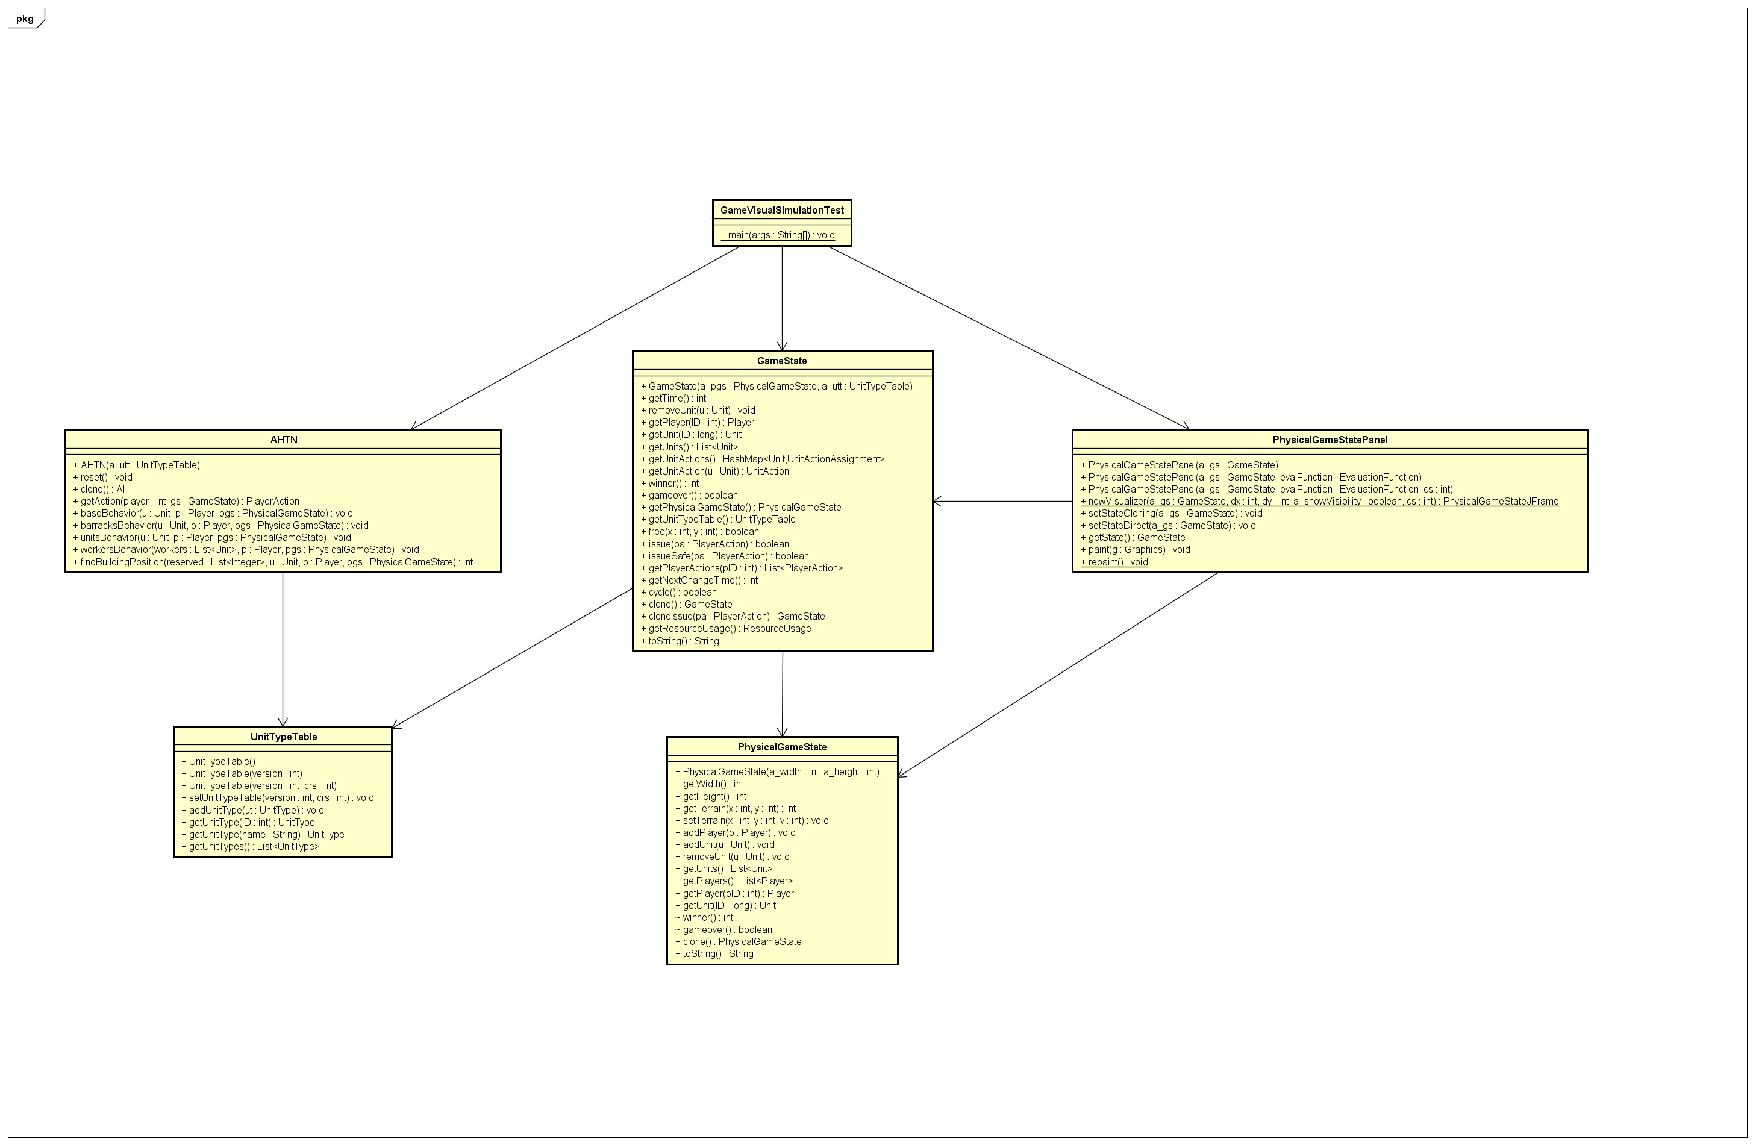
\includegraphics[width=0.7\textwidth]{fig/classes.pdf}
  	\caption{Classes do MicroRTS}
  	\label{fig:classes}
  \end{figure} 


\section{Cronograma}

Para a próxima etapa do projeto do Trabalho de Conclusão, foi proposto o plano das atividades apresentado no diagrama de Gantt com a respectiva legenda.

\begin{itemize}
\item Tarefa 1 - Escrita do TC II.
\item Tarefa 2 - Desenvolvimento do dominio.
\item Tarefa 3.1 - Implementação do algoritmo AHTN.
\item Tarefa 3.2 - Testar e corrigir possíveis erros da implementação.
\item Tarefa 4 - Criação dos \textit{benchmark}.
\item Tarefa 5 - Integrar o algoritmo de \textit{q-learning} a implementação. 
\item Tarefa 6 - Realizar a comparação com as outras abordagens. 
\item Tarefa 7 - Preparar a apresentação. 
\end{itemize}

\begin{ganttchart}{1}{21}
	\gantttitle{Volume Final TCI}{21} \\
	\gantttitlelist{6,...,12}{3} \\
	\ganttgroup{TC II}{6}{20} \\	
	\ganttmilestone{Entrega do volume Final TCI}{3} \ganttnewline	
	\ganttbar{Tarefa 1}{7}{20} \\	
	\ganttbar{Tarefa 2}{7}{8} \\
	\ganttbar{Tarefa 3.1}{9}{10} \\	
	\ganttbar{Tarefa 3.2}{11}{12} \\	
	\ganttbar{Tarefa 4}{13}{14} \\
	\ganttbar{Tarefa 5}{15}{16} \\
	\ganttbar{Tarefa 6}{17}{18} \\	
	\ganttbar{Tarefa 7}{19}{20} \\	
	\ganttmilestone{Entrega Volume Final}{20} \ganttnewline
	%\ganttlinkedgroup{Task 3}{2}{3}
	%\ganttlinkedbar{Task 3}{3}{7} \ganttnewline
%	%\ganttmilestone{Milestone}{7} \ganttnewline
%	%\ganttbar{Final Task}{8}{12}	
%	\ganttlink{elem2}{elem8}
%	\ganttlink{elem5}{elem6}	
%	\ganttlink{elem3}{elem6}
%	\ganttlink{elem4}{elem7}
%	\ganttlink{elem6}{elem7}
%	\ganttlink{elem8}{elem9}
\end{ganttchart}



%----------------------------------------------------------------
% Aqui vai a bibliografia. Existem 3 estilos de citação: use
% 'tcc-alpha' para citações do tipo [Abc+] ou [XYZ] (em ordem
% alfabética na bibliografia), 'tcc-num' para citações
% numéricas do tipo [1], [20], etc., em ordem de referência e
% 'tcc-alpha-full' para citações estilo 'alpha' mas com nomes completos.
%----------------------------------------------------------------
%\bibliographystyle{tcc-alpha}
%\frm[inline]{A citação para o Russel e Norvig está errada, para que o título é o autor!!}
\bibliographystyle{tcc-num}
\bibliography{referencias}

%----------------------------------------------------------------
% Após \appendix, se iniciam os capítulos de Apêndice, com
% numeração alfabética.
%----------------------------------------------------------------
%\appendix
%\chapter{Meu primeiro apêndice}
%\chapter{My second appendix}

%----------------------------------------------------------------
% Aqui vão os "capítulos" de anexos. Cada anexo deve
% ser considerado um capítulo.
%----------------------------------------------------------------
%\anexos
%\chapter{Meu primeiro anexo}
%\chapter{My second attachment}

% E aqui (para a felicidade de todos) termina o documento.
\end{document}
